We have seen in Chapter~\ref{chap:lattice} two independant methods to create
lattices of compatibly embedded finite fields. In this chapter, we present a new
framework, inspired by both Conway polynomials and Bosma-Canon-Steel, that we
call \emph{standard lattice of compatibly embedded finite fields}.
\minitoc

% TODO: Figure

\clearpage

\section{Lenstra-Allombert algorithm and lattices of embeddings}
\label{sec:lenstra-allombert-embeddings}

The two methods of Chapter~\ref{chap:lattice} both have their drawbacks: Conway
polynomials are expensive to compute and thus need to be precomputed, making
them inefficient for large extensions, while Bosma-Canon-Steel needs more
computation each time an embedding is added in the lattice. % Not precise enough/!\
Our starting point in order to propose an alternative framework for lattices of
compatibly embedded finite fields is Lenstra-Allombert algorithm and the study
of Kummer algebras done in Section~\ref{sec:kummer-algebras}. In all this
chapter, $\K=\mathbb{F}_p$ is a prime field of cardinality $p$, where
$p\in\mathbb{N}$ is a prime number.

\subsection{From isomorphism to embedding}
\label{sec:iso-to-emb}

Let us first recall Lenstra-Allombert \emph{isomorphism} algorithm. We keep the
notations of Section~\ref{sec:allombert}, where the details can be found. Let $K$ and
$L$ be two finite fields with $p^n$ elements, where $\gcd(p, n) = 1$, \ie
\[
  p\nmid n.
\]
We know that $K$ and $L$ are isomorphic and, if $\zeta$ is a primitive $n$-th
root of unity taken in the algebraic closure $\bar{\mathbb{F}}_p$ of $\K$, we know
% Note:
% =====
%
% We did not speak about algebraic closure in Chapter 5, where we introduce the
% notions of isomorphisms and algorithms to compute them. It is probably wise
% not to introduce that here only.
we can find an isomorphism by
finding two solutions $\alpha_K$ and $\alpha_L$ to the equation~\eqref{eq:h90-kummer}
\[
  (\sigma\otimes1)(\alpha) = (1\otimes\zeta)\alpha,
\]
respectively in $K\otimes\mathbb{F}_p(\zeta)$ and $L\otimes\mathbb{F}_p(\zeta)$.
We then compute $\kappa\in\mathbb{F}_p(\zeta)$ such that
\[
  1\otimes\kappa^n = \alpha_K^n/\alpha_L^n
\]
and the map
\[
  \phi:\first{\alpha_K}{\zeta}\mapsto\first{(1\otimes\kappa)\alpha_L}{\zeta}
\]
is then an isomorphism from $K$ to $L$. A key part of the algorithm is that the
root $\zeta$ must be the same in the two Kummer algebras
$K\otimes\mathbb{F}_p(\zeta)$ and $L\otimes\mathbb{F}_p(\zeta)$. In practice, it
means that we need to use elements that have the same minimal polynomial to
define $\zeta$ in both algebras. This constraint might seem easy to fulfill in
this case, but it becomes harder in the case of a \emph{compatible embedding}
computation. Assume that $m, n\in\mathbb{N}$ are two integers such that
\[
  m\mid n
\]
and $\gcd(p, m)=\gcd(p, n)=1$. Let $K$ be a finite field with $p^m$ elements and
$L$ a finite fields with $p^n$ elements. We know that $K$ is isomorphic to a
subfield of $L$, \ie we have an embedding
\[
  K\emb L.
\]
To compute an embedding, one solution is to compute the algebras
$K\otimes\mathbb{F}_p(\zeta_m)$ and
$L\otimes\mathbb{F}_p(\zeta_m)$, where $\zeta_m$ is a primitive $m$-th root of
unity, as done in the isomorphism case, then compute solutions
$\alpha_{K, m}, \alpha_{L, m}$ of~\eqref{eq:h90-kummer} and the constant
$\kappa=\kappa_{K\emb L}$. This solution is satisfying as long as we only want
to compute a \emph{single} embedding in $L$. Indeed, assume we also have an
integer $l\in\mathbb{N}$ that divides $n$, such that $\gcd(p, l)=1$, and a
finite field $H$ of cardinality $p^l$. Then there is an embedding
\[
  H\emb L,
\]
and in order to compute it we must find a primitive $l$-th root of unity
$\zeta_l$, compute $L\otimes\mathbb{F}_p(\zeta_l)$, compute a new solution
$\alpha_{L, l}$ of~\eqref{eq:h90-kummer} for $\zeta_l$ and the associated
constant $\kappa_{H\emb L}$. Therefore, each new embedding comes with the
computation of a new Kummer algebra, a new solution of~\eqref{eq:h90-kummer}, and a
new element $\kappa$. We must also store the elements $\kappa$ and the elements
defining the embeddings. Now, recall that if we want to use Bosma-Canon-Steel
framework in order to compatibly embed $K$ in $L$, we must reccursively embed
the intersection $K\cap M$ in both fields $K$ and $M$, for each already
embedded subfield $M$ of $L$. 
\begin{center}
  \begin{tikzpicture}
    \node (K) at (0, 2) {$K$};
    \node (L) at (2, 4) {$L$};
    \node (M) at (4, 2) {$M$};
    \node (I) at (2, 0) {$K\cap M$};
    \node (?) at (1, 1) {\textbf{?}};
    \node (??) at (3, 1) {\textbf{?}};

    \draw[dashed-arrow] (K) to (L);
    \draw[arrow] (M) to (L);
    \draw[possible-arrow] (I) to (K);
    \draw[possible-arrow] (I) to (M);
  \end{tikzpicture}
\end{center}
This yields a quadratic memory complexity in the number of extensions in the
lattice and their degrees, as well as a quadratic number of new embedding
computations, \ie computations of Kummer algebras and solutions
of~\eqref{eq:h90-kummer}. It motivates a new solution with only one computation
of Kummer algebra and~\eqref{eq:h90-kummer} solution per extension in the lattice,
independently of the number of embedded subfields. Assume we have $\zeta_m$ and
$\zeta_n$ respectively two $m$-th and $n$-th primitive roots
of unity that are \emph{compatible}, \ie such that
\[
  (\zeta_n)^{n/m} = \zeta_m.
\]
We compute the Kummer algebras $K\otimes\mathbb{F}_{p}(\zeta_m)$ and
$L\otimes\mathbb{F}_p(\zeta_n)$, $\alpha_K$ a solution of~\eqref{eq:h90-kummer}
for the root $\zeta_m$ and $\alpha_L$ a solution of~\eqref{eq:h90-kummer} for
the root $\zeta_n$. In that case, the element
\[
  (\alpha_L)^{n/m}\in L\otimes\mathbb{F}_p(\zeta_n)
\]
is a solution of~\eqref{eq:h90-kummer} for the root $(\zeta_n)^{n/m}=\zeta_m$,
indeed
\begin{align*}
  (\sigma\otimes1)((\alpha_L)^{n/m}) &=
  ( (\sigma\otimes1)(\alpha_{L}))^{n/m} \\
  &= ( (1\otimes\zeta_n)\alpha_L)^{n/m}\\
  &= (1\otimes (\zeta_n)^{n/m})(\alpha_L)^{n/m}.
\end{align*}
The embedding $K\emb L$ is then described by
\[
  \first{\alpha_K}{\zeta_m}\mapsto\first{(1\otimes\kappa_{K\emb
  L})(\alpha_L)^{n/m}}{(\zeta_n)^{n/m}},
\]
where $\kappa_{K\emb L}\in\mathbb{F}_p(\zeta_n)$ is a $m$-th root of
$\alpha_L^n/\alpha_K^m$. There are still two issues with such a solution. First,
it is still necessary to store the constants $\kappa_{K\emb L}$ for each
embedding
\[
  K\emb L
\]
in the lattice. We would like these constants $\kappa$ to be equal to $1$, or
maybe that a close formula exists for these constants, by choosing special
solutions $\alpha$ of~\eqref{eq:h90-kummer}. We achieve the latter
by constructing \emph{standard} solutions of~\eqref{eq:h90-kummer} in
Section~\ref{sec:standard-solution}.

\subsection{Cyclotomic lattices}

The second, and most important, issue is the compatibility condition between the
roots of unity $\zeta$. When we write a compatibility condition like
\[
  \zeta_m = (\zeta_n)^{n/m},
\]
we implicitly states that there is a natural inclusion 
\[
  \mathbb{F}_p(\zeta_m)\subseteq\mathbb{F}_p(\zeta_n)
\]
that makes the embedding from $\mathbb{F}_{p}(\zeta_m)$ to
$\mathbb{F}_{p}(\zeta_n)$ trivial, \ie the embedding is the identity in that
case. In practice, this is not always the situation at hand. For example,
if for some reason the root $\zeta_m$ already exists in some field
$\mathbb{F}_{p^a}$ in the current state of our computer algebra system, and if the
root $\zeta_n$ lives in a strictly bigger field
$\mathbb{F}_{p^b}=\mathbb{F}_p(\zeta_n)$ that we have to compute, then the field
$\mathbb{F}_{p^a}$ is not included in the field $\mathbb{F}_{p^b}$, and the
embedding
\[
  \mathbb{F}_{p^a}\emb \mathbb{F}_{p^b}
\]
is not trivial. In the general case, if we want to use Lenstra-Allombert
embedding algorithm, what we need is a \emph{cyclotomic
lattice}, given by Definition~\ref{defi:cyclotomic-lattice}.
\begin{defi}[Cyclotomic lattice]
  \label{defi:cyclotomic-lattice}
  A \emph{cyclotomic lattice} is composed of two things:
  \begin{itemize}
    \item a collection
  \[
    \mathcal S^I = \left\{ (K_m, \zeta_m) \right\}_{m\in I}
  \]
  over some support set $I\subset \mathbb{N}\setminus p\mathbb{N}$. The element
  $K_m$ is an explicitly represented finite extension of $\K=\mathbb{F}_p$, and
  the element $\zeta_m\in K_m$ is a generating element of $K_m$ that is also a
  primitive $m$-th root of unity, \ie we have
  \[
  K_m = \mathbb{F}_{p}(\zeta_m)
  \]
  and
  \[
  (\zeta_m)^m=1.
  \]
    \item explicit embeddings
      \[
        \begin{array}{llll}
          \iota_{m, n}: & K_m & \emb & K_n\\
          & \zeta_m & \mapsto & (\zeta_n)^{n/m}
        \end{array}
      \]
      whenever $(m, n)\in I^2$ are such that $m\mid n$.
  \end{itemize}
\end{defi}

Again, there is no problem if we know beforehand all the degrees of the
extensions in the lattice that we will use, \ie if the support set $I$ is
finite. Indeed, in that case there is an efficient randomised algorithm to
compute the cyclotomic lattice: consider
\[
  N = \lcm_{m\in I}(m)
\]
and construct the smallest finite field $\mathbb{F}_{p^a}$ such that $N$ divides
$p^a-1$, \ie the smallest finite field containing an $N$-th primitive root of
unity. Then take $x\in\mathbb{F}_{p^a}$ at random, compute 
\[
  y=x^{(p^a-1)/N}
\]
and check that the multiplicative order of $y$ is $N$. If it is, we can
construct all roots $\zeta_m$ as powers of this element:
\[
  \zeta_m = y^{N/m}
\]
for all $m\in I$, and we can set
\[
  K_m = \mathbb{F}_p(\zeta_m)\subset \mathbb{F}_{p^a}
\]
and let the embeddings $\iota_{m, n}$ be natural inclusions. But once again,
this methode does not produce an incremental lattice, thus it is not really user
friendly: one would like to have a lattice where new elements can be added on
the fly. Conway polynomials, that were introduced in
Section~\ref{sec:conway} in order to construct a lattice of
compatibly embedded finite fields, offer an other example of cyclotomic lattice. In
fact, a cyclotomic lattice is always a lattice of compatibly embedded finite
fields, because each time we have $l, m, n\in I$ with
\[
  l\mid n\mid n,
\]
we have
\[
  (\zeta_n)^{n/l} = ((\zeta_n)^{m/l})^{n/m}
\]
and it follows that
\[
  \iota_{l, n} = \iota_{m, n}\circ\iota_{l, m}.
\]
One can thus wonder why we need a structure than can be used to represent a
lattice of compatibly embedded finite fields, precisely to construct a lattice
of compatibly embedded finite fields. In fact, we will see in the next sections
that with a fairly small cyclotomic lattice, we are able to construct a much larger
lattice of compatibly embedded finite fields, thus making the whole construction
interesting, above all if the cyclotomic lattice is incrementable, like with
Conway polynomials. In the next sections, we consider that we have an abstract
cyclotomic lattice, without precising any particular construction. We only
assume that we have a collection $\mathcal S^I$ satisfying the conditions of
Definition~\ref{defi:cyclotomic-lattice}.

\subsection{Kummer embeddings}
\label{sec:kummer-embeddings}

As we have seen in the last sections, asking for a compatibility condition
\[
  \zeta_m = (\zeta_n)^{n/m}
\]
each time we want to use Lenstra-Allombert embedding algorithm to embed
$\mathbb{F}_{p^m}$ in $\mathbb{F}_{p^n}$, in a compatible way, is not trivial:
it requires the availability of a cyclotomic lattice. Moreover, this equation
implies that there is a natural inclusion
\[
  \mathbb{F}_{p}(\zeta_m)\subset\mathbb{F}_{p}(\zeta_n),
\]
which is not the case in general. In order to be as thorough as possible, we
will thus write
\[
  \iota_{m, n}(\zeta_m) = (\zeta_{n})^{n/m}
\]
and generalize the discussion of Section~\ref{sec:iso-to-emb} and the results of
Section~\ref{sec:lenstra-allombert-isomorphism} in this setting. We keep the
``Kummer algebra'' terminology, already used in
Section~\ref{sec:kummer-algebras}, that is based on~\cite{DRR19}. We know assume
that a cyclotomic lattice $\mathcal S^I$ is available. Let
\[
  m\mid n
\]
be two integers prime to $p$, we then have an embedding
\[
\begin{array}{cccc}
  \iota_{m, n}: & \mathbb{F}_{p}(\zeta_m)& \emb &\mathbb{F}_{p}(\zeta_n)\\
  & \zeta_m & \mapsto & (\zeta_n)^{n/m}.
\end{array}
\]
We also let
\[
  A_m=\mathbb{F}_{p^m}\otimes\mathbb{F}_{p}(\zeta_m)
\]
and
\[
  A_n=\mathbb{F}_{p^n}\otimes\mathbb{F}_{p}(\zeta_n)
\]
be two Kummer algebras. As was the case for
Lenstra-Allombert \emph{isomorphism} algorithm, we want to deduce a field
embedding from an algebra embedding between $A_m$ and $A_n$, using the
properties of the solutions of~\eqref{eq:h90-kummer}. We are thus
interested in a special class of morphisms that are closely linked with
these solutions.
\begin{defi}[Kummer embedding]
  \label{defi:kummer-embedding}
  A \emph{Kummer embedding} of $A_m$ into $A_n$ is an injective
  $\K$-algebra morphism
  \[
    \Phi:A_m\emb A_n
  \]
  such that:
  \begin{itemize}
    \item the morphism $\Phi$ extends the scalar embedding
      $1\otimes\iota_{m,n}$;
    \item the morphism $\Phi$ commutes with $\sigma\otimes1$.
  \end{itemize}
\end{defi}
We can in fact give a simpler characterization of Kummer embeddings, and see that
they are of the form $\Phi=\phi\otimes\iota$, where $\iota$ is the embedding
described by the cyclotomic lattice $\mathcal S^I$. The embedding $\phi$ is then the one for
which we will try to obtain a description, using the properties of the solutions
of~\eqref{eq:h90-kummer}.
\begin{prop}
  \label{prop:correspondence-embeddings}
  There is a $1$-to-$1$ correspondence between Kummer embeddings
  \[
    \Phi:A_m\emb A_n
  \]
  and embeddings of finite fields
  \[
    \phi:\mathbb{F}_{p^m}\emb\mathbb{F}_{p^n},
  \]
  given by:
  \begin{itemize}
    \item if $\Phi$ is a Kummer embedding, then $\Phi$ maps
      $\mathbb{F}_{p^m}\otimes1$ into $\mathbb{F}_{p^n}\otimes1$. Thus the
      restriction of $\Phi$ to $\mathbb{F}_{p^m}$ is of the form $\phi\otimes1$
      for some embedding $\phi:\mathbb{F}_{p^m}\emb\mathbb{F}_{p^n}$, and we
      have $\Phi=\phi\otimes\iota_{m, n}$;
    \item conversely, if $\phi:\mathbb{F}_{p^m}\emb\mathbb{F}_{p^n}$ is an
      embedding of finite fields, then $\Phi=\phi\otimes\iota_{m, n}$ is a
      Kummer embedding.
  \end{itemize}
  In conclusion, the correspondence is given by
  \[
    \Phi=\phi\otimes\iota_{m, n}\longleftrightarrow \phi.
  \]
  Moreover, this correspondence commutes with composition of embeddings.
\end{prop}
\begin{proof}
 Let $\Phi:A_m\emb A_n$ be a Kummer embedding. Since $\Phi$ is an algebra
 morphism, we have 
 \[
   \Phi(\beta^p) = \Phi(\beta)^p
 \]
for all $\beta\in A_m$. Since $(\sigma\otimes\sigma)(\beta) = \beta^p$, this
proves that $\Phi$ commutes with $\sigma\otimes\sigma$. It also
commutes with $\sigma\otimes1$, and thus with its inverse $\sigma^{-1}\otimes1$.
It then also commutes with
\[
  (\sigma^{-1}\otimes1)\circ(\sigma\otimes\sigma) = 1\otimes\sigma.
\]
Now, if $\beta\in\mathbb{F}_{p^m}\otimes1$, we know thanks
to Remark~\ref{rem:fixed-elems} that it is fixed by $1\otimes\sigma$, thus we have that
\begin{align*}
 (1\otimes\sigma)\circ\Phi(\beta) &= \Phi\circ(1\otimes\sigma)(\beta)\\
 &= \Phi(\beta).
\end{align*}
Again, using Remark~\ref{rem:fixed-elems}, we then know that
$\Phi(\beta)\in\mathbb{F}_{p^n}\otimes1$. This proves that
$\mathbb{F}_{p^m}\otimes1$ is mapped into $\mathbb{F}_{p^n}\otimes1$. Now, it
means that every element of the form $x\otimes1$ with $x\in\mathbb{F}_{p^m}$ is
mapped to an element of the form $\Phi(x\otimes1)=y\otimes1$ with $y\in\mathbb{F}_{p^m}$.
Because $\Phi$ is a morphism of algebras, if we
let $\phi(x)=y$, we can check that
\[
  \phi:\mathbb{F}_{p^m}\to\mathbb{F}_{p^n}
\]
is also a morphism. Therefore, the restriction of $\Phi$ on
$\mathbb{F}_{p^m}$ is of the form $\phi\otimes1$, where
$\phi:\mathbb{F}_{p^m}\emb\mathbb{F}_{p^n}$ is an embedding
of finite fields. We conclude that $\Phi=\phi\otimes\iota_{m, n}$. Indeed, if 
\[
  \beta=\sum_{j}x_j\otimes y_j
\]
is an element of the Kummer algebra $A_m$, we then have
\begin{align*}
  \Phi(\beta) &= \Phi(\sum_{j}x_j\otimes y_j) \\
  &= \sum_j\Phi(x_j\otimes y_j)\\
  &= \sum_j\Phi(x_j\otimes1)\times\Phi(1\otimes y_j)\\
  &= \sum_j(\phi\otimes1)(x_j\otimes1)\times(1\otimes\iota_{m, n})(1\otimes y_j)\\
  &= \sum_j (\phi(x_j)\otimes1)\times(1\otimes\iota_{m, n}(y_j))\\
  &= \sum_j \phi(x_j)\otimes\iota_{m, n}(y_j)\\
  &= \sum_j (\phi\otimes\iota_{m, n})(x_j\otimes y_j)\\
  &= (\phi\otimes\iota_{m, n})(\sum_jx_j\otimes y_j),
\end{align*}
and thus
\[
  \Phi(\beta) = (\phi\otimes\iota_{m, n})(\beta)
\]
for every element $\beta\in A_m$.

Conversely, if $\phi:\mathbb{F}_{p^{m}}\emb\mathbb{F}_{p^n}$ is an embedding of
finite fields and if we define
\[
  \Phi = \phi\otimes\iota_{m, n},
\]
we see that $\Phi$ is a morphism of $\K$-algebras that extends the scalar embedding
$\iota_{m, n}$ by definition.
The embedding $\phi$ is a power of the Frobenius automorphism $\sigma$ and thus
commutes with $\sigma$, hence $\sigma\otimes1$ commutes with
$\Phi=\phi\otimes\iota_{m, n}$, and this proves that $\Phi$ is a Kummer
embedding.

Now, if we have three Kummer algebras $A_l, A_m, A_n$ such that 
\[
  l\mid m\mid n
\]
and two Kummer embeddings $\Phi_{l, m}:A_l\emb A_m$ and $\Phi_{m, n}:A_m\emb
A_n$, we know that there exists $\phi_{l,
m}:\mathbb{F}_{p^l}\emb\mathbb{F}_{p^m}$ and $\phi_{m,
n}:\mathbb{F}_{p^{m}}\emb\mathbb{F}_{p^{n}}$ such that we have the following
diagram.
\begin{center}
    \begin{tikzpicture}
      \node (l) at (0, 0) {$A_l$};
      \node (m) at (0, 1.5) {$A_m$};
      \node (n) at (0, 3) {$A_n$};

      \draw[arrow] (l) -- (m);
      \draw[arrow] (m) -- (n);

      \node (f12) at (2, 0.65)
      {$\Phi_{l,m}=\phi_{l, m}\otimes\iota_{l, m}$};
      \node (f13) at (2, 2.15)
      {$\Phi_{m,n}=\phi_{m, n}\otimes\iota_{m, n}$};
    \end{tikzpicture}
\end{center}
Now the map $\Phi_{m, m}\circ\Phi_{l,m}$ is a Kummer embedding from $A_l$ into
$A_n$, hence there exist an embedding
$\phi:\mathbb{F}_{p^{l}}\emb\mathbb{F}_{p^{n}}$ such that 
\[
  \Phi_{m, m}\circ\Phi_{l,m}=\phi\otimes\iota_{l, n}.
\]
But we also have 
\[
  \Phi_{m, m}\circ\Phi_{l,m}=(\phi_{m, n}\circ\phi_{l,
  m})\otimes(\iota_{m, n}\circ\iota_{l, m}),
\]
and since $\iota_{l,n}=\iota_{m, n}\circ\iota_{l, m}$ by definition, we obtain
\[
  \phi_{m, n}\circ\phi_{l, m}=\phi,
\]
thus the correspondence commutes with compositions of embeddings.
\end{proof}
\begin{prop}
  \label{prop:correspondence-solutions}
  Let $\alpha_m\in A_m$ be a nonzero solution of~\eqref{eq:h90-kummer} for
  $\zeta_m$, and let $c_m$ be its Kummer constant. Then, there is a $1$-to-$1$
  correspondence between Kummer embeddings
  \[
    \Phi:A_l\emb A_m
  \]
  and solutions $\hat\alpha\in A_n$ of~\eqref{eq:h90-kummer} for
  $(\zeta_n)^{n/m}=\iota_{m, n}(\zeta_m)$ that also satisfy
  \[
    \hat\alpha^m = 1\otimes\iota_{m, n}(c_m).
  \]
  The correspondence is given by
  \[
    \Phi(\alpha_m)\longleftrightarrow \hat\alpha.
  \]
\end{prop}
\begin{proof}
Let $\Phi:A_m\emb A_n$ be a Kummer embedding. Lemma~\ref{lm:h90-solutions} shows
that $\alpha_m$ is a generator of $A_m$ as an $1\otimes\mathbb{F}_{p}(\zeta_m)$
algebra. Thus every element $\beta\in A_m$ can be written in the form
\[
  \beta = \sum_{j=0}^{m-1}(1\otimes b_j)(\alpha_m)^j,
\]
and we obtain
\[
  \Phi(\beta) = \sum_{j=0}^{m-1}(1\otimes\iota_{m, n}(b_j))\Phi(\alpha_m)^j,
\]
therefore we see that $\Phi$ is determined by its image $\Phi(\alpha_m)$. Moreover,
$\hat\alpha=\Phi(\alpha_m)$ is a solution of~\eqref{eq:h90-kummer} for
$(\zeta_n)^{n/m}=\iota_{m,n}(\zeta_m)$ that satisfies
$\hat\alpha^m=\iota_{m, n}(c_m)$. Indeed, this is a generalization of the
computations done in Section~\ref{sec:kummer-algebras} and a consequence of
Definition~\ref{defi:kummer-embedding}. We have
\begin{align*}
 (\sigma\otimes1)(\hat\alpha) &=(\sigma\otimes1)(\Phi(\alpha_m))\\
 &= \Phi( (\sigma\otimes1)(\alpha_m))\\
 &= \Phi((1\otimes\zeta_m)\alpha_m)\\
 &= (1\otimes\iota_{m, n})(\zeta_m)\Phi(\alpha_m)\\
 &= (1\otimes\iota_{m, n}(\zeta_m))\hat\alpha
\end{align*}
and
\begin{align*}
 \hat\alpha^m &= \Phi(\alpha_m)^m\\
 &= \Phi(\alpha_m^m)\\
 &= \Phi(1\otimes c_m)\\
 &= 1\otimes\iota_{m, n}(c_m).
\end{align*}

 Converserly, if $\hat\alpha$ is a solution of~\eqref{eq:h90-kummer} for
 $\iota_{m, n}(\zeta_m)$ such that $\hat\alpha^m=\iota_{m, n}(c_m)$, we see that
 \[
  \Phi(\beta) = \sum_{j=0}^{m-1}(1\otimes\iota_{m, n}(b_j))\hat\alpha^j,
 \]
 for any element
 \[
  \beta = \sum_{j=0}^{m-1}(1\otimes b_j)(\alpha_m)^j
 \]
 gives a well-defined morphism of algebras from  $A_m$ into $A_n$ that satisfies
 $\Phi(\alpha)=\hat\alpha$ and
 the conditions in Definition~\ref{defi:kummer-embedding}, \ie it extends
 $\iota_{m, n}$ and commutes with $\sigma\otimes1$.
\end{proof}
With these two correspondences, we can now describe a little more the link
between solutions of~\eqref{eq:h90-kummer} and the finite field embeddings
$\phi$ that we compute from them.
\begin{cor}
  \label{cor:link-h90-embedding}
  Let $\alpha_m\in A_m$ be a nonzero solution of~\eqref{eq:h90-kummer} for
  $\zeta_m$ with Kummer constant $c_m$ and let $\hat\alpha\in A_n$ be a solution
  of~\eqref{eq:h90-kummer} for $(\zeta_n)^{n/m}$ that satisfies
  $\hat{\alpha}^m=\iota_{m, n}(c_m)$. Then
  \begin{itemize}
    \item the solution $\hat{\alpha}$ belongs to the subset
      $\mathbb{F}_{p^{l}}\otimes\mathbb{F}_p((\zeta_n)^{n/m})\subset A_n$;
    \item the assignation
      $\first{\alpha_m}{\zeta_m}\mapsto\first{\hat\alpha}{(\zeta_n)^{n/m}}$
      defines an embedding $\phi:\mathbb{F}_{p^{m}}\emb\mathbb{F}_{p^{n}}$;
    \item the map $\Phi=\phi\otimes\iota_{m, n}$ is the unique Kummer embedding
      such that $\Phi(\alpha_m)=\hat\alpha$.
  \end{itemize}
\end{cor}
\begin{proof}
  By Proposition~\ref{prop:correspondence-solutions}, we know that there exists
  a unique Kummer embedding 
  \[
    \Phi:A_m\emb A_n
  \]
  such that $\Phi(\alpha_m) =
  \hat\alpha$. We also know thanks to
  Proposition~\ref{prop:correspondence-embeddings} that
  \[
    \Phi=\phi\otimes\iota_{m, n}
  \]
  for some embedding of finite fields
  $\phi:\mathbb{F}_{p^{m}}\emb\mathbb{F}_{p^{n}}$. If $\alpha_m =
  \sum_{j=0}^{a-1}x_j\otimes(\zeta_m)^j$, where $a$ is the level of $A_m$, we
  obtain
  \[
    \hat\alpha = \sum_{j=0}^{a-1}\phi(x_j)\otimes(\zeta_n)^{\frac{in}{m}},
  \]
  thus we have $\hat\alpha\in\mathbb{F}_{p^{m}}\otimes\mathbb{F}_{p}(
  (\zeta_n)^{n/m})$. We also see that $x_0=\first{\alpha_m}{\zeta_m}$ is mapped
  to $\phi(x_0) = \first{\hat\alpha}{(\zeta_n)^{n/m}}$, but
  $\first{\alpha_m}{\zeta_m}$ is a generating element of
  $\mathbb{F}_{p^{m}}$ by Proposition~\ref{prop:generate}, hence the assignation
  \[
    \first{\alpha_m}{\zeta_m}\mapsto\first{\hat\alpha}{(\zeta_n)^{n/m}}
  \]
  defines $\phi$.
\end{proof}
With these results we are ready to generalize
Proposition~\ref{prop:lenstra-allombert-algorithm} to the embedding case, with
the cyclotomic lattice setting, giving a minor variation of the original
algorithm of Allombert.
\begin{algorithm}
  \caption{(Allombert's algorithm)}
  \label{algo:allombert}
  \begin{algorithmic}[1]
    \Require{$\mathbb{F}_{p^m}, \mathbb{F}_{p^n}$, for $m\mid n$ integers prime to $p$,
    and a cyclotomic lattice $\mathcal S^{\{l,m\}}$.}
    \Ensure{$s\in \mathbb{F}_{p^m}, t\in\mathbb{F}_{p^n}$, such that the assignation $s\mapsto t$
    defines an embedding $\phi:\mathbb{F}_{p^{m}}\emb\mathbb{F}_{p^n}$.}
  \State Construct the Kummer algebras $A_m$ and $A_n$.
  \State Find $\alpha_m\in A_m$ and $\alpha_n\in A_n$, nonzero solutions
  of~\eqref{eq:h90-kummer} for $\zeta_m$
  and $\zeta_n$ respectively.
  \State Compute their Kummer constants: $(\alpha_m)^m=1\otimes c_m$ and
  $(\alpha_n)^n=1\otimes c_n$.
  \State Compute $\kappa$, a $m$-th root of $\iota_{m, n}(c_m)/c_n$.
  \State Return $\first{\alpha_{m}}{\zeta_m}$ and
  $\first{(1\otimes\kappa)(\alpha_n)^{\frac{n}{m}}}{(\zeta_n)^{\frac{n}{m}}}$.
  \end{algorithmic}
\end{algorithm}
\begin{prop}
  \label{prop:allombert-works}
  Algorithm~\ref{algo:allombert} is correct: it returns elements that define an
  embedding $\phi:\mathbb{F}_{p^{m}}\emb\mathbb{F}_{p^{n}}$.
\end{prop}
\begin{proof}
  The ideas of the proof are the same as the ones found in the proof of
  Proposition~\ref{prop:lenstra-allombert-algorithm}, which were already present
  in the simpler case of Proposition~\ref{prop:allombert-simple}, where all the
  roots of unity are in $\K$. By
  Proposition~\ref{prop:correspondence-embeddings}, let 
  \[
    \Phi=\phi\otimes\iota_{m, n}
  \]
  be a Kummer embedding from $A_m$ into $A_n$. Let $\alpha_m\in A_m$ a solution
  of~\eqref{eq:h90-kummer} for $\zeta_m$ with Kummer constant $c_m$, and let
  $\alpha_n\in A_n$ a solution of~\eqref{eq:h90-kummer} for $\zeta_n$ with
  Kummer constant $c_n$. By
  Proposition~\ref{prop:correspondence-solutions}, there is a solution $\hat\alpha\in
  A_n$ of~\eqref{eq:h90-kummer} for $(\zeta_n)^{n/m}$ that satisfies
  $\hat{\alpha}^m=\iota_{m, n}(c_m)$ and such that $\Phi(\alpha_m)=\hat\alpha$.
  Now, we also have that $(\alpha_n)^{n/m}$ is a solution
  of~\eqref{eq:h90-kummer} for $(\zeta_n)^{n/m}$, and the solutions
  of~\eqref{eq:h90-kummer} for $(\zeta_n)^{n/m}$ form a one-dimensional
  $1\otimes\mathbb{F}_{p}(\zeta_n)$-vector space, so there exists a constant
  $\lambda\in\mathbb{F}_{p}(\zeta_n)$ such that
  \[
    \hat\alpha = (1\otimes\lambda)(\alpha_n)^{n/m}.
  \]
  We conclude that 
  \[
    \cfrac{\iota_{m, n}(c_m)}{c_n} = \lambda^m
  \]
  is a $m$-th root in $\mathbb{F}_{p}(\zeta_n)$. If we let
  \[
    \kappa = (\zeta_n)^{\frac{in}{m}}\lambda,
  \]
  for some integer $i$, be a $m$-th root of $\frac{\iota_{m, n}(c_m)}{c_n}$, it
  follows that
  \[
    \tilde\alpha = (1\otimes\kappa)(\alpha_n)^{n/m} =
    (1\otimes(\zeta_n)^{\frac{in}{m}})\hat\alpha
  \]
  is a solution of~\eqref{eq:h90-kummer} for $(\zeta_n)^{n/m}$ that satisfies
  $\tilde\alpha^m = \iota_{m,n}(c_m)$. By
  Corollary~\ref{cor:link-h90-embedding}, we know that the assignation
  \[
    \first{\alpha_m}{\zeta_m}\mapsto\first{\tilde\alpha}{(\zeta_n)^{n/m}}
  \]
  defines an embedding from $\mathbb{F}_{p^m}$ into $\mathbb{F}_{p^{n}}$.
\end{proof}
\begin{rem}
  Taking the same notations as the one in the proof of
  Proposition~\ref{prop:allombert-works}, we see that the embedding returned by
  the algorithm is $\sigma^i\circ\phi$. Indeed, we have
  \begin{align*}
    \tilde\alpha &= (1\otimes(\zeta_n)^{\frac{in}{m}})\hat\alpha\\
    &= (\sigma\otimes1)^i(\hat\alpha)\\
    &= (\sigma^i\otimes1)(\hat\alpha).
  \end{align*}
  If we let $x_0=\first{\hat\alpha}{(\zeta_n)^{\frac{n}{m}}}$, we wee that the
  returned embedding is defined by the assignation
  \[
    \first{\alpha_m}{\zeta_m}\mapsto\sigma^i(x_0)
  \]
  while $\phi$ is defined by
  \[
    \first{\alpha_m}{\zeta_m}\mapsto x_0.
  \]
\end{rem}
\section{Standard solution of Hilbert $90$}
\label{sec:standard-solution}

\subsection{Complete algebras and standardization}
\label{sec:standardization}

We discussed in Section~\ref{sec:iso-to-emb} the 
obstacles when constructing a lattice of compatibly embedded finite fields using
Lenstra-Allombert algorithm. The first one is that we need to have compatibility
between the roots of unity that we use, and that can be hard to obtain in
practice. We solved that problem by assuming the availability of a
cyclotomic lattice $\mathcal S^I$, and we proved that all the results concerning
Lenstra-Allombert can be expressed in that setting in
Section~\ref{sec:kummer-embeddings}. Now, we can obtain compatibility by
replacing the naive embedding algorithm by Lenstra-Allombert algorithm in
Bosma-Canon-Steel framework. This solutions immediately gives a compatible
lattice of embedded finite fields. Still, among the sub-goals presented in
Section~\ref{sec:compatibility-problem} that such a lattice may achieve, there
are two of them on which we would like to improve.
\begin{description}
  \item[\emph{Uniqueness:}] the element $\first{\lambda_m}{\zeta_m}$ is
    a generator of $\mathbb{F}_{p^{m}}$, or equivalently, it provides an
    irreducible polynomial in $\K[X]$ of degree $m$. However this polynomials
    depends on the choice of $\alpha_l$, because it depends on the Kummer constant
    $c_l$ of $\alpha_l$ by Proposition~\ref{prop:kummer-constant}, thus there is
    no uniqueness.
  \item[\emph{Compatibility:}] the embedding of finite fields
    $\phi:\mathbb{F}_{p^{m}}\to\mathbb{F}_{p^{n}}$ depends on
    the choice of the constant $\kappa$, which itself depends on the choice of
    the solutions $\alpha_m$ and $\alpha_n$ of \eqref{eq:h90-kummer}, and also
    of the choice of a $m$-th root of unity. In order to achieve compatibility,
    we must keep track of the constants $\kappa$ for each embedding computation
    \[
      \mathbb{F}_{p^{m}}\emb\mathbb{F}_{p^{n}}
    \]
    in the
    lattice, which grow quadratically with the number of fields, because of the
    common subfield compatibility condition in Bosma-Canon-Steel framework.
\end{description}
In this section and in Section~\ref{sec:standard-embeddings}, we will see how to
choose special solutions of \eqref{eq:h90-kummer}, in order to manage these
constants $\kappa$. Our dream would be to be able to choose the solutions
of~\eqref{eq:h90-kummer} in a way that makes the constants trivial, \ie 
\[
  \kappa_{\mathbb{F}_{p^{m}}\emb \mathbb{F}_{p^{n}}} = 1.
\]
From Algorithm~\ref{algo:allombert}, we see that the constant
$\kappa_{\mathbb{F}_{p^{m}}\emb\mathbb{F}_{p^{n}}}$ is a $m$-th root of the
quotient
\[
  \cfrac{\iota_{m, n}(c_m)}{c_n},
\]
thus the condition $\kappa_{\mathbb{F}_{p^{m}}\emb\mathbb{F}_{p^{n}}}=1$ implies
\[
  \iota_{m, n}(c_m) = c_n,
\]
which in turn implies that $c_n$ belongs to the subset
\[
  \mathbb{F}_{p}( (\zeta_n)^{\frac{n}{m}})\subseteq\mathbb{F}_p(\zeta_n).
\]
This could possibly fail if the Kummer algebras $A_m$ and $A_n$ are of distinct
level, \ie if their field of scalars are different. This motivates the study of
Kummer algebras of a given level, and the introduction of the notion of
\emph{complete} algebra.
\begin{defi}[Complete Kummer algebra]
  A Kummer algebra is \emph{complete} if it is of the largest degree for a given
  level.
\end{defi}
Therefore, the complete Kummer algebra of level $a$ is the Kummer algebra
\begin{align*}
  A_{p^a-1} &=
  \mathbb{F}_{p^{p^a-1}}\otimes\mathbb{F}_p(\zeta_{p^a-1})\\
  &=\mathbb{F}_{p^{p^a-1}}\otimes\mathbb{F}_{p^{a}}
\end{align*}
with field of scalar
\[
  \mathbb{F}_{p^{a}}\cong \mathbb{F}_p(\zeta_{p^a-1}).
\]
given by the element $\zeta_{p^a-1}$ in the cyclotomic lattice $\mathcal S^I$.
In fact these algebras have an interesting property.
\begin{lm}
  All nonzero solutions $\alpha_{p^a-1}\in A_{p^a-1}$ of~\eqref{eq:h90-kummer}
  for $\zeta_{p^a-1}$ have the same Kummer constant
  \[
    c_{p^a-1} = (\zeta_{p^a-1})^{a}.
  \]
\end{lm}
\begin{proof}
  \label{lm:complete-algebra-solutions}
  Let $\alpha_{p^a-1}\in A_{p^a-1}$ a solution of~\eqref{eq:h90-kummer} for
  $\zeta_{p^a-1}$. For all $\beta\in A_{p^a-1}$, we have $\beta^p = \sigma\otimes\sigma(\beta) =
  \beta^p$, so we also obtain 
  \[
    (\alpha_{p^a-1})^{p^a} = (\sigma^a\otimes\sigma^a)(\alpha_{p^a-1}).
  \]
  Now, we know that $\sigma^a$ is the identity on $\mathbb{F}_{p^a}$, hence we
  have
  \begin{align*}
    (\alpha_{p^a-1})^{p^a} &= (\sigma^a\otimes1)(\alpha_{p^a-1}) \\
    &= (1\otimes\zeta_{p^a-1})^a \alpha_{p^a-1}.
  \end{align*}
  Since $\alpha_{p^a-1}$ is invertible by Lemma~\ref{lm:h90-solutions}, we
  obtain that
  \[
    (\alpha_{p^a-1})^{p^a-1} = 1\otimes c_{p^a-1} = (1\otimes \zeta_{p^a-1})^a
  \]
  and it follows that
  \[
    c_{p^a-1} = (\zeta_{p^a-1})^{a}.
  \]
\end{proof}
Now this result is very important because we know that the degree $p^a-1$
irreducible polynomial in $\K[X]$ derived from the solution $\alpha_{p^a-1}$,
\ie the minimal polynomial of the element
$\first{\alpha_{p^a-1}}{\zeta_{p^a-1}}$,
only depends on the Kummer constant $c_{p^a-1}$ of $\alpha_{p^a-1}$, thus it
means that all solutions give the same polynomial. This will be the central idea
behind the notion of \emph{standard} elements.
\begin{defi}[Standard Kummer constant]
  Let $m$ be an integer prime to $p$. We define the \emph{standard Kummer
  constant} of order $m$ as
  \[
    \stdc{m} = (\iota_{m,
    p^a-1})^{-1}((\zeta_{p^a-1})^a)\in\mathbb{F}_{p}(\zeta_m),
  \]
  where $a=\nu(m)$ is the level of the Kummer algebra $A_m$.
\end{defi}
\begin{rem}
 Since $A_m$ is of level $a$, we have
 \[
   \mathbb{F}_p(\zeta_m) \cong \mathbb{F}_p(\zeta_{p^a-1}),
 \]
 hence the map $\iota_{m, p^a-1}$ is an isomorphism and $\stdc{m}$ is
 well-defined.
\end{rem}
\begin{defi}[Standard solution]
  Let $m$ be an integer prime to $p$. We say that a solution $\alpha_m\in A_m$
  is \emph{standard} if its Kummer constant is standard, \ie if we have
  \[
    (\alpha_m)^m = 1\otimes\stdc{m}.
  \]
\end{defi}
\begin{defi}[Decorated Kummer algebra]
  Let $m$ be an integer prime to $p$. We define a \emph{decorated Kummer
  algebra} as a couple
  \[
    (A_m, \alpha_m),
  \]
  where $\alpha_m$ is a standard solution of~\eqref{eq:h90-kummer} for
  $\zeta_m$.
\end{defi}
It follows from Lemma~\ref{lm:complete-algebra-solutions} that all nonzero
solutions of~\eqref{eq:h90-kummer} in a complete algebra are standard. This is
no longer the case in a non complete Kummer algebra, but we can still find
standard solutions.
\begin{prop}
  \label{prop:decoration}
 Let $m$ an integer prime to $p$. Then $A_m$ can be decorated, \ie it admits a
 standard solution $\alpha_m$. Moreover, this solution $\alpha_m$ is unique up
 to a $m$-th root of unity. 
\end{prop}
\begin{proof}
 Let $a=\nu(m)$ be the level of $A_m$ and let $\alpha_m'\in A_m$ be a nonzero solution
 of~\eqref{eq:h90-kummer} for $\zeta_m$. Let also $\alpha_{p^a-1}$ be a nonzero
 solution of~\eqref{eq:h90-kummer} for $\zeta_{p^a-1}$, then it is standard by
 Lemma~\ref{lm:complete-algebra-solutions}. The element 
 \[
   (\alpha_{p^a-1})^{\frac{p^a-1}{m}}
 \]
 is a solution of~\eqref{eq:h90-kummer} for
 \[
   \iota_{m, p^a-1}(\zeta_m) = (\zeta_{p^a-1})^{\frac{p^a-1}{m}}.
 \]
 Now let
 \[
   \Phi:A_m\emb A_{p^a-1}
 \]
 be a Kummer embedding and let
 \[
   \hat\alpha = \Phi(\alpha_m'),
 \]
 then $\hat\alpha$ is also a solution of~\eqref{eq:h90-kummer} for
 $\iota_{m, p^a-1}(\zeta_m)$ and thus there exists a scalar
 $\lambda\in\mathbb{F}_p(\zeta_{p^a-1})$ such that
 \[
   (\alpha_{p^a-1})^{\frac{p^a-1}{m}} = (1\otimes\lambda)\hat{\alpha} .
 \]
 If we let
 \[
   \tilde\lambda = \iota_{m, p^a-1}^{-1}(\lambda),
 \]
 we obtain
 \begin{align*}
   (\alpha_{p^a-1})^{\frac{p^a-1}{m}} &= (1\otimes\lambda)\Phi(\alpha_m') \\
   &= \Phi( (1\otimes\tilde\lambda)\alpha_m').
 \end{align*}
If we set 
\[
  \alpha_m = (1\otimes\tilde\lambda)\alpha_m',
\]
it follows that
\begin{align*}
  \Phi((\alpha_m)^m) &= (\alpha_{p^a-1})^{p^a-1} \\
  &= 1\otimes(\zeta_{p^a-1})^a,
\end{align*}
therefore
\begin{align*}
  (\alpha_m)^m &= 1\otimes\iota_{m, p^a-1}^{-1}( (\zeta_{p^a-1})^a) \\
  &= 1 \otimes \stdc{m}
\end{align*}
and $\alpha_m$ is standard. If $\beta\in A_m$ is another solution
of~\eqref{eq:h90-kummer} for $\zeta_m$, then there exists a scalar
$\mu\in\mathbb{F}_p(\zeta_m)$ such that
\[
  \alpha_m= (1\otimes\mu)\beta,
\]
but then we obtain
\[
  (\alpha_m)^m = (1\otimes\mu^m)\beta^m.
\]
As a consequence, $\beta$ is standard if and only if $\mu^m = 1$ and the
standards solutions are the
\[
  (1\otimes\zeta_m^u)\alpha_m
\]
for $0\leq u\leq m-1$.
\end{proof}
From Proposition~\ref{prop:decoration}, it follows that for any integer $m$
prime to $p$, we can define $\mathbb{F}_{p^{m}}$ in a standard way.
\begin{defi}[Standard generating element]
  A generating element $x\in\mathbb{F}_{p^{m}}$ is called \emph{standard} if it
  is of the form
  \[
    x = \first{\alpha_m}{\zeta_m}
  \]
  for $\alpha_m\in A_m$ a standard solution of~\eqref{eq:h90-kummer}.
\end{defi}
\begin{defi}[Standard defining polynomial]
  The \emph{standard defining polynomial} $P_m$ for $\mathbb{F}_{p^{m}}$ is the
  minimal polynomial over $\K$ of a standard generating element of
  $\mathbb{F}_{p^{m}}$.
\end{defi}
\begin{defi}[Decorated finite field]
  Let $m\in\mathbb{N}$ an integer prime to $p$. A \emph{decorated finite field}
  is a couple $(\mathbb{F}_{p^{m}}, s_m)$ where $s_m\in\mathbb{F}_{p^{m}}$ is a
  standard generating element.
\end{defi}
\begin{rem}
  By Remark~\ref{rem:recover-alpha}, we can recover $\alpha_m$ the standard
  solution of~\eqref{eq:h90-kummer} from the standard generating element $s_m$,
  thus decorated Kummer algebras can be recovered from
  decorated finite fields.
\end{rem}
By Proposition~\ref{prop:kummer-constant}, we know that $P_m$ is entirely 
determined by $\stdc{m}$, and thus by the cyclotomic lattice $\mathcal S^I$ up
to order $p^a-1$, with $a=\nu(m)$ the level of $m$. This helps to achieve the
\emph{uniqueness} sub-goal of our lattice, because once the cyclotomic lattice
has been chosen, the standard defining polynomials are unique. As an example, we
give in Table~\ref{tab:std-polys} the first ten standard defining polynomials
induced by the cyclotomic lattice given by the Conway polynomials with $p=2$.
\begin{table}
  \centering
  \begin{tabular}{l}
    $x+1$ \\
    $x^3+x+1$ \\
    $x^5+x^3+1$ \\
    $x^7+x+1$ \\
    $x^9+x^7+x^4+x^2+1$\\
    $x^{11}+x^8+x^7+x^6+x^2+x+1$\\
    $x^{13}+x^{10}+x^5+x^3+1$\\
    $x^{15}+x+1$ \\
    $x^{17}+x^{11}+x^{10}+x^8+ x^7+x^6+x^4+x^3+x^2+x+1$ \\
    $x^{19}+x^{17}+x^{16}+x^{15}+x^{14}+x^{13}+x^{12}+x^8+x^7+x^6+x^5+x^3+1$
  \end{tabular}
  \caption{The first ten standard polynomials derived from Conway
    polynomials for $p=2$.}
  \label{tab:std-polys}
\end{table}
A small variation of Lenstra-Allombert algorithm, given by
Algorithm~\ref{algo:decoration}, allows us to compute all these standard
elements.
\begin{algorithm}
  \caption{(Decoration -- Standardization)}
  \label{algo:decoration}
  \begin{algorithmic}[1]
    \Require {$\mathbb{F}_{p^m}$, for $m$ prime to $p$, and $\mathcal{S}^I$ a cyclotomic lattice.}
    \Ensure {$(A_m,\alpha_m)$ decorated, $P_m$ standard irreducible polynomial of degree $m$,
      and $s\in\mathbb{F}_{p^m}$ standard generating element inducing $\mathbb{F}_{p^m}\simeq\mathbb{F}_{p}[T]/(P_m)$.}
  \State Compute the Kummer algebra $A_m$.
  \State Compute $\stdc{m}=(\iota_{m, p^a-1})^{-1}((\zeta_{p^a-1})^a)\in\mathbb{F}_p(\zeta_m)$.
  \State Find $\alpha'_m\in A_m$ a nonzero solution of~\eqref{eq:h90-kummer} for $\zeta_m$.
  \State Compute its Kummer constant: $(\alpha'_m)^m=1\otimes c'_m$.
  \State Compute $\kappa$ a $m$-th root of $\stdc{m}/ c'_m$.
  \State Set $\alpha_{m}=(1\otimes\kappa)\alpha'_m$.
  \State Compute $P_m$ the minimal polynomial of $\first{\alpha_{m}}{\zeta_m}$
  over $\K$.
  \State Return $(A_m,\alpha_m)$, $P_m$, and $\first{\alpha_m}{\zeta_m}$.
  \end{algorithmic}
\end{algorithm}
\begin{prop}
  Algorithm~\ref{algo:decoration} is correct, \ie the computed element
  $\alpha_m$ is indeed standard. 
\end{prop}
\begin{proof}
  By Proposition~\ref{prop:decoration}, we know that there exists a standard
  solution of~\eqref{eq:h90-kummer} for $\zeta_m$, let $\pmb{\alpha}\in A_m$ be such a
  solution. Let $\alpha_m'\in A_m$ be any nonzero solution
  of~\eqref{eq:h90-kummer} for $\zeta_m$ and let $c_m'$ be its Kummer constant.
  Then we know that there exists $\lambda\in\mathbb{F}_p(\zeta_m)$ a scalar such that
  \[
    \pmb\alpha = (1\otimes\lambda)\alpha_m'.
  \]
  It follows that 
  \[
    \stdc{m} = \lambda^m c_m',
  \]
  thus 
  \[
    \stdc{m}/c_m'
  \]
  is indeed a $m$-th power. If we let $\kappa$ be a $m$-th root of
  $\stdc{m}/c_m'$ and if we set 
  \[
    \alpha_m = (1\otimes\kappa)\alpha_m',
  \]
  we obtain
  \[
    (\alpha_m)^m = 1\otimes\stdc{m}.
  \]
  We have thus proven that $\alpha_m$ is a standard solution
  of~\eqref{eq:h90-kummer} for $\zeta_m$. By definition,
  $\first{\alpha_m}{\zeta_m}$ is then a standard generating element of
  $\mathbb{F}_{p^{m}}$ and its minimal polynomial $P_m$ is a standard defining
  polynomial.
\end{proof}

\subsection{Towards standard embeddings}
\label{sec:towards-standard-embeddings}

Now that we have found a way to compute standard solutions
of~\eqref{eq:h90-kummer}, and to deduce standard generating elements to define
our finite fields, it is natural to work towards the definition of compatible
embeddings between these finite fields that are also standard. Our goal is also
to simplify the storage of the constants $\kappa$ involved in the computation of
such embeddings.
\begin{prop}
  \label{prop:power-compatibility}
  Let $m\mid n$ be two integers prime to $p$ and such that 
  \[
    \nu(m) = \nu(n),
  \]
  \ie the (decorated) Kummer algebras $(A_m, \alpha_m)$ and $(A_n, \alpha_n)$
  have the same level. Then there is a unique Kummer embedding
  \[
    \stdemb{m}{n}:A_m\emb A_n
  \]
  such that
  \[
    \stdemb{m}{n}(\alpha_m) = (\alpha_n)^{\frac{n}{m}}.
  \]
\end{prop}
\begin{proof}
  The element $\hat\alpha = (\alpha_n)^{\frac{n}{m}}$ is a solution
  of~\eqref{eq:h90-kummer} for $(\zeta_n)^{\frac{n}{m}}=\iota_{m, n}(\zeta_m)$.
  We also know that the Kummer constant of $\alpha_m$ is
  \[
    \stdc{m} = \iota_{m, p^a-1}^{-1}((\zeta_{p^a-1})^a)
  \]
  and the Kummer constant of $\alpha_n$ is 
  \[
    \stdc{n} = \iota_{n, p^a-1}^{-1}((\zeta_{p^a-1})^a).
  \]
  The embeddings $\iota$ are compatible by definition, thus we have
  \[
    \iota_{m, p^a-1} = \iota_{n, p^a-1}\circ\iota_{m, n}
  \]
  and
  \[
    \iota_{n, p^a-1}^{-1} = \iota_{m, n}\circ\iota_{m, p^a-1}^{-1}.
  \]
  It follows that
  \[
    \stdc{n} = \iota_{m, n}(\stdc{m}).
  \]
  By Proposition~\ref{prop:correspondence-solutions}, there exists a unique
  Kummer embedding $\stdemb{m}{n}$ such that
  \[
    \stdemb{m}{n}(\alpha_m) = \hat\alpha = (\alpha_n)^{\frac{n}{m}}.
  \]
\end{proof}
Proposition~\ref{prop:power-compatibility} guarantees that decorated Kummer
algebras $(A_m, \alpha_m), (A_n, \alpha_n)$ of the same level are
\emph{power-compatible}, \ie we can describe a unique Kummer embedding by
\[
  \alpha_m\mapsto (\alpha_n)^{\frac{n}{m}}.
\]
Therefore, there is no constant $\kappa$ to store in this case because we are in
the trivial case $\kappa=1$, which was our
goal. However, we see that power compatibility implies
\[
  \stdc{n} = \iota_{m, n}(\stdc{m}),
\]
hence implies that the decorated Kummer algebras share the same level. If the
Kummer algebras do not share the same level, we can ask for
\emph{norm-compatibility} instead of power-compatibility, at least between two
\emph{complete} decorated Kummer algebras. 
Let us first describe what ``norm'' we will be using.
Let $A_n$ be a Kummer algebra of level $\nu(n) = b$, so that
\[
  A_n = \mathbb{F}_{p^{n}}\otimes\mathbb{F}_{p^{b}}\cong
  \mathbb{F}_{p^{n}}\otimes\mathbb{F}_{p}(\zeta_{p^b-1}),
\]
where the isomorphism is given by $1\otimes\iota_{n, p^b-1}$. Then, if $a\mid b$
is another integer, the subalgebra of $A_n$ invariant under $1\otimes\sigma^a$
is identified (by the same isomorphism) with
\[
  (A_n)^{1\otimes\sigma^a} \cong \mathbb{F}_{p^{n}}\otimes\mathbb{F}_p(
  (\zeta_{p^b-1})^{\frac{p^b-1}{p^a-1}})
\]
where
\[
  (\zeta_{p^b-1})^{\frac{p^b-1}{p^a-1}} =
  N_{\mathbb{F}_{p^{n}}/\mathbb{F}_{p^{a}}}(\zeta_{p^b-1}) = \iota_{p^a-1,
  p^b-1}(\zeta_{p^a-1})
\]
and where $N_{\mathbb{F}_{p^{n}}/\mathbb{F}_{p^{a}}}$ is the relative norm of
the finite field extension
\[
  \mathbb{F}_{p^{b}}/\mathbb{F}_{p^{a}}.
\]
\begin{defi}[Scalar norm operator]
  Let $n$ an integer prime to $p$ and $A_n$ a Kummer algebra of level
  $\nu(n)=c$. Let $a,b$ two integers such that $a\mid b \mid c$,
  then we define the \emph{scalar norm operator} as
  \[
    \begin{array}{cccc}
      \mathcal N_{b/a,\, A_n}: & (A_n)^{1\otimes\sigma^b} & \to &
      (A_n)^{1\otimes\sigma^a}\\
      & \gamma & \mapsto & \prod_{0\leq j\leq
        \frac{a}{b}}(1\otimes\alpha^{ja})(\gamma)
    \end{array}
  \]
\end{defi}
This operator is well-defined, as the elements in the image of $\mathcal
N_{b/a,\, A_n}$ are indeed invariant under $1\otimes\sigma^a$. We often 
omit $A_n$ and only write $\N_{b/a}$, as the ambient space $A_n$ is
implicit. By construction, $\N_{b/a}$ acts on the scalar field
$1\otimes\mathbb{F}_{p^b}^\times$ as the usual norm $1\otimes
N_{\mathbb{F}_{p^{b}}/\mathbb{F}_{p^{a}}}$. Scalar norms are
\emph{multiplicative}, \ie for any $\gamma, \gamma'\in A_n$, we have
\[
  \N_{b/a}(\gamma\gamma') = \N_{b/a}(\gamma)\N_{b/a}(\gamma'),
\]
they are \emph{transitive}, \ie for any $a\mid b\mid c$, we have
\[
  \N_{c/a} = \N_{b/a}\circ\N_{c/b},
\]
and they commute with $\sigma\otimes1$. All these nice properties make the
scalar norm an excellent candidate to generalize the powering used to define
standard embeddings between decorated Kummer algebras of same level.
\begin{prop}
  \label{prop:norm-compatibility}
  Let $a\mid b$ be two integers prime to $p$ and let $(A_{p^a-1},
  \alpha_{p^a-1})$, $(A_{p^b-1}, \alpha_{p^b-1})$ two decorated complete
  Kummer algebras of levels $a$ and $b$ respectively. Then there is a unique
  Kummer embedding (that we again call \emph{standard})
  \[
    \stdemb{p^a-1}{p^b-1}:A_{p^a-1}\emb A_{p^b-1}
  \]
  such that
  \[
    \stdemb{p^a-1}{p^b-1}(\alpha_{p^a-1}) = \N_{b/a}(\alpha_{p^b-1}).
  \]
\end{prop}
\begin{proof}
  Let $\hat\alpha = \N_{b/a}(\alpha_{p^b-1})$, by the properties of the scalar
  norm, we have
  \begin{align*}
    (\sigma\otimes1)(\hat\alpha) &=
    (\sigma\otimes1)(\N_{b/a}(\alpha_{p^b-1}))\\
    &= \N_{b/a}( (\sigma\otimes1)(\alpha_{p^b-1}))\\
    &= \N_{b/a}( (1\otimes\zeta_{p^b-1})\alpha_{p^b-1})\\
    &= (1\otimes(\zeta_{p^b-1})^{\frac{p^b-1}{p^a-1}})\N_{b/a}(\alpha_{p^b-1}),
  \end{align*}
  therefore $\hat\alpha$ is a solution of~\eqref{eq:h90-kummer} for
  $(\zeta_{p^b-1})^{\frac{p^b-1}{p^a-1}}$.
  We also have 
  \begin{align*}
    \hat\alpha^{p^a} &= (\sigma^a\otimes\sigma^a)(\hat\alpha)\\
    &= (\sigma^a\otimes\sigma^a)(\N_{b/a}(\alpha_{p^b-1}))\\
    &= (\sigma^a\otimes1)(\N_{b/a}(\alpha_{p^b-1}))\\
    &= \N_{b/a}((\sigma^a\otimes1)(\alpha_{p^b-1}))\\
    &= \N_{b/a}((1\otimes(\zeta_{p^b-1})^a)(\alpha_{p^b-1}))\\
    &= (1\otimes\iota_{p^a-1,\,p^b-1}(\zeta_{p^a-1})^a)\N_{b/a}(\alpha_{p^b-1}),
  \end{align*}
  thus $\hat\alpha$ satisfies
  \[
    \hat\alpha^{p^a-1} = 1\otimes\iota_{p^a-1,\,p^b-1}(\stdc{p^a-1}),
  \]
  and by Proposition~\ref{prop:correspondence-solutions} there is a unique
  embedding such that
  \[
    \stdemb{p^a-1}{p^b-1}(\alpha_{p^b-1}) = \hat\alpha.
  \]
\end{proof}

\section{Standard embeddings}
\label{sec:standard-embeddings}

From Proposition~\ref{prop:power-compatibility}, we learned how to construct a
standard Kummer embedding between two decorated Kummer algebras sharing the same
level, using power compatibility. From Proposition~\ref{prop:norm-compatibility}
we learned how to construct a standard Kummer embedding between two decorated
complete Kummer algebras, using norm compatibility. Our goal is
now to use both results together in order to construct a standard Kummer
embedding between any two decorated Kummer algebras. Consider the general
case where we have two integers
$m\mid n$ not divisible by $p$, set $a=\nu(m)$, $b=\nu(n)$, and consider
the diagram
\begin{equation*}
\label{3cotes}
\begin{CD}
(A_{p^a-1},\alpha_{p^a-1}) @>{\stdemb{p^a-1}{p^b-1}}>> (A_{p^b-1},\alpha_{p^b-1}) \\
@A{\stdemb{m}{p^a-1}}AA @AA{\stdemb{n}{p^b-1}}A\\
(A_m,\alpha_m) @. (A_n,\alpha_n)
\end{CD}
\end{equation*}
of standard embeddings of decorated algebras.
\begin{lm}
  \label{lm:existence-embedding}
  In this setting, there exists a unique Kummer embedding
  \[
    \stdemb{m}{n}:A_m\emb A_n
  \]
  that makes the diagram commute. We call this embedding the \emph{standard
  Kummer embedding} from $A_m$ to $A_n$.
\end{lm}
\begin{proof}
  Let
  \[
    \tilde\alpha = \stdemb{p^a-1}{p^b-1}(\stdemb{m}{p^a-1}(\alpha_l))\in
    A_{p^b-1}.
  \]
  The element $\tilde\alpha$ is fixed by both $\sigma^m\otimes1$ and
  $1\otimes\sigma^a$, because $\alpha_m$ is, and Kummer embeddings commute with both
  $\sigma\otimes1$ and $1\otimes\sigma$. Therefore, $\tilde\alpha$ is also fixed
  by $\sigma^n\otimes1$ and $1\otimes\sigma^b$, and thus is in the image of
  $A_n$ by $\stdemb{n}{p^b-1}$. We then let
  \[
    \hat\alpha = (\stdemb{n}{p^b-1})^{-1}(\tilde\alpha)\in A_n.
  \]
  By construction, the element $\tilde\alpha$ is a solution
  of~\eqref{eq:h90-kummer} for
  \[
    \iota_{m,\,p^b-1}(\zeta_m) = (\zeta_{p^b-1})^{\frac{p^b-1}{m}}
  \]
  that satisfies
  \[
    \tilde\alpha^m = 1\otimes\iota_{m,\,p^b-1}(\stdc{m})
  \]
  It thus follows that $\hat\alpha$ is a solution
  of~\eqref{eq:h90-kummer} for 
  \[
    \iota_{n,\,p^b-1}^{-1}(\iota_{m,\,p^b-1}(\zeta_m)) =
    \iota_{m\,n}(\zeta_m)=(\zeta_n)^{\frac{n}{m}}
  \]
  that also satisfies 
  \[
    \hat\alpha^m = 1\otimes\iota_{m,n}(\stdc{m}).
  \]
  By Proposition~\ref{prop:correspondence-solutions}, we then have a unique
  Kummer embedding such that
  \[
    \stdemb{m}{n}(\alpha_m) = \hat\alpha,
  \]
  and that concludes the proof.
\end{proof}
\begin{defi}[Standard embedding]
  Let $m\mid n$ two integers prime to $p$. By
  Proposition~\ref{prop:correspondence-embeddings}, there exists a unique finite
  field embedding 
  \[
    \stdembff{m}{n}:\mathbb{F}_{p^{m}}\emb\mathbb{F}_{p^{n}}
  \]
  such that the standard Kummer embedding $\stdemb{m}{n}$ satisfies
  \[
    \stdemb{m}{n}=\stdembff{m}{n}\otimes\iota_{m,n}.
  \]
  This finite field embedding $\stdembff{m}{n}$ is called the \emph{standard embedding}
  from $\mathbb{F}_{p^{m}}$ to $\mathbb{F}_{p^{n}}$.
\end{defi}
The existence result of Lemma~\ref{lm:existence-embedding} is 
``constructive'', but requires to compute the complete Kummer algebra
$A_{p^a-1}$, that can be very large, thus it is impractical. However, one should
be able to write 
\[
  \hat\alpha = (1\otimes\kappa)(\alpha_n)^{\frac{n}{m}}
\]
for some constant $\kappa\in\mathbb{F}_p(\zeta_n)$,
since both $\hat\alpha$ and $(\alpha_n)^{\frac{n}{m}}$ are solutions
of~\eqref{eq:h90-kummer} for $(\zeta_n)^\frac{n}{m}$. We proved in
Lemma~\ref{lm:existence-embedding} that there was a unique, \emph{standard},
Kummer embedding corresponding to this solution $\hat\alpha$, thus there should
also be a unique constant $\kappa$ corresponding to this embedding. Our aim is
now to give an explicit expression of $\kappa$, so that we do not have to
compute the complete algebra $A_{p^b-1}$ to obtain the Kummer embedding
\[
  \stdemb{m}{n}.
\]
We start with the simpler case of complete algebras nonetheless, \ie we study
the constant $\kappa$ when $m=p^a-1$ and $n=p^b-1$.
\begin{prop}
  \label{prop:link-norm-power}
In the complete algebra $A_{p^b-1}$ we have
\[
(\alpha_{p^b-1})^{\frac{p^b-1}{p^a-1}}=(1\otimes\zeta_{p^b-1})^{\frac{(b-a)
  p^{b+a}-bp^b+ap^a}{(p^a-1)^2}}\norm_{b/a}(\alpha_{p^b-1}).
\]
\end{prop}
\begin{proof}
  Using the fact that $(\sigma\otimes\sigma)(\beta) = \beta^p$ for any $\beta\in
  A_{p^b-1}$, and then~\eqref{eq:h90-kummer}, we get:
  \begin{align*}
\frac{(\alpha_{p^b-1})^{\frac{p^b-1}{p^a-1}}}{\norm_{b/a}(\alpha_{p^b-1})}
&=\prod_{0\leq j<\frac{b}{a}}\frac{(\sigma^{ja}\otimes\sigma^{ja})(\alpha_{
p^b-1})}{(1\otimes\sigma^{ja})(\alpha_{p^b-1})}\\
&=\prod_{0\leq j<\frac{b}{a}}(1\otimes\sigma^{ja})\left(\frac{(\sigma^{ja}
\otimes 1)(\alpha_{p^b-1})}{\alpha_{p^b-1}}\right)\\
&=\prod_{0\leq j<\frac{b}{a}}(1\otimes\sigma^{ja})(1\otimes\zeta_{p^b-1})
^{ja}\\
&=(1\otimes\zeta_{p^b-1})^{\sum_{0\leq j<\frac{b}{a}}jap^{ja}}.
  \end{align*}
We conclude thanks to the identity
\[
\sum_{0\leq j<n}jT^j=T\frac{d}{dT}\!\left(\frac{T^n-1}{T-1}\right)=
\frac{(n-1)T^{n+1}-nT^n+T}{(T-1)^2}.
\]
\end{proof}
From Proposition~\ref{prop:link-norm-power}, we can deduce the constant $\kappa$
involved in the computation of $\stdemb{p^a-1}{p^b-1}$. The results also extends
to non complete algebras.
\begin{cor}
  \label{cor:link-norm-power}
  Let $(A_m, \alpha_n)$ and $(A_n, \alpha_n)$ be two decorated Kummer algebras
  of respective degrees $m\mid n$ prime to $p$ and respective levels $a$ and
  $b$. Then the standard embedding
  \[
    \stdemb{m}{n}:A_m\emb A_n
  \]
  is defined by the assignation
  \[
    \alpha_m\mapsto (1\otimes\kappa_{m, n})(\alpha_n)^{\frac{n}{m}},
  \]
  where 
  \[
    \kappa_{m, n} = \iota_{n,
    p^b-1}^{-1}(\zeta_{p^b-1})^{-\frac{(b-a)p^{b+a}-bp^b+ap^a}{(p^a-1)m}}.
  \]
\end{cor}
\begin{proof}
  Recall that $\stdemb{m}{n}$ is, by construction, the unique Kummer embedding
  that makes the following diagram commute.
\begin{equation*}
\begin{CD}
(A_{p^a-1},\alpha_{p^a-1}) @>{\stdemb{p^a-1}{p^b-1}}>> (A_{p^b-1},\alpha_{p^b-1}) \\
@A{\stdemb{m}{p^a-1}}AA @AA{\stdemb{n}{p^b-1}}A\\
(A_m,\alpha_m) @. (A_n,\alpha_n)
\end{CD}
\end{equation*}
Therefore, if we set
\[
  \hat\alpha = (1\otimes\kappa_{m, n})(\alpha_n)^{\frac{n}{m}},
\]
it is sufficient, by Lemma~\ref{lm:existence-embedding}, to prove that 
\[
  \stdemb{p^a-1}{p^b-1}(\stdemb{m}{p^b-1})(\alpha_m) =
  \stdemb{n}{p^b-1}(\hat\alpha).
\]
However, using Proposition~\ref{prop:norm-compatibility} and
Proposition~\ref{prop:power-compatibility}, we know that
\[
  \stdemb{p^a-1}{p^b-1}(\stdemb{m}{p^b-1})(\alpha_m) =
  \norm_{b/a}(\alpha_{p^b-1})^{\frac{p^a-1}{m}},
\]
and we also know that
\[
  \stdemb{n}{p^b-1}( (\alpha_m)^{\frac{n}{m}}) =
  (\alpha_{p^b-1})^{\frac{p^b-1}{m}}.
\]
Therefore, using Proposition~\ref{prop:link-norm-power}, we obtain
\begin{align*}
  \stdemb{n}{p^b-1}(\hat\alpha) &=   (\zeta_{p^b-1})^{-\frac{(b-a)p^{b+a}
-bp^b+ap^a}{(p^a-1)m}}(\alpha_{p^b-1})^{\frac{p^b-1}{m}}\\
&=( (\zeta_{p^b-1})^{-\frac{(b-a)p^{b+a}
-bp^b+ap^a}{(p^a-1)^2}}(\alpha_{p^b-1})^{\frac{p^b-1}{p^a-1}})^{\frac{p^a-1}{m}}\\
&= \norm_{b/a}(\alpha_{p^b-1})^{\frac{p^a-1}{m}}\\
&= \stdemb{p^a-1}{p^b-1}(\stdemb{m}{p^b-1})(\alpha_m),
\end{align*}
which completes the proof.
\end{proof}
\begin{prop}
  \label{prop:embeddings-compatibility}
  Standard Kummer embeddings are compatible: let $(A_l, \alpha_l), (A_m,
  \alpha_m)$ and $(A_n, \alpha_n)$ three decorated Kummer algebras with
  respective degrees
  \[
    l\mid m\mid n,
  \]
  then the corresponding standard embeddings satisfy
  \[
    \stdemb{l}{n} = \stdemb{m}{n}\circ\stdemb{l}{m}.
  \]
\end{prop}
\begin{proof}
  Corollary~\ref{cor:link-norm-power} gives us explicit formulas for the
  standard Kummer embeddings, thus we can check by direct computation that the
  embeddings are compatible. Let
  \[
    a = \nu(l)\quad b =\nu(m)\quad c = \nu(n)
  \]
  the respective levels of $A_l, A_m$ and $A_n$. Then we have the corresponding
  commutative diagram where the arrows represent the standard Kummer embeddings.
 \begin{equation*}
\begin{CD}
A_{p^a-1} @>>> A_{p^b-1} @>>> A_{p^c-1} \\
@AAA @AAA @AAA\\
A_l @>>> A_m @>>> A_n
\end{CD}
\end{equation*} 
Using Lemma~\ref{lm:existence-embedding}, it is sufficient to show that
\[
  \stdemb{l}{n}(\alpha_l)
\]
and
\[
  (\stdemb{m}{n}\circ\stdemb{l}{m})(\alpha_l)
\]
have the same image in $A_{p^c-1}$ under $\stdemb{n}{p^c-1}$. However, it
follows from the diagram that this common image is 
\[
  \norm_{c/a}(\alpha_{p^c-1})^{\frac{p^a-1}{l}}.
\]
\end{proof}
All these results ensure that Algorithm~\ref{algo:std-embed} is correct and
provides embeddings that are compatible.
\begin{algorithm}
  \caption{(Standard compatible embeddings)}
  \label{algo:std-embed}
  \begin{algorithmic}[1]
    \Require {$\mathcal S^I$ a cyclotomic lattice, and
      $(\mathbb{F}_{p^m},s_m)$, $(\mathbb{F}_{p^n},s_n)$, decorated finite
    fields, for $m\mid n$ integers prime to $p$.}
      \Ensure {$t\in\mathbb{F}_{p^n}$, such that the assignation $s_m\mapsto t$
    defines a standard embedding
    $\stdembff{m}{n}:\mathbb{F}_{p^m}\hookrightarrow\mathbb{F}_{p^n}$,
      compatible with composition.}
  \State Compute the Kummer algebras $A_m$ and $A_n$.
  \State Recover $\alpha_m$ from $s_m$ and $\alpha_n$ from $s_n$ using
  Remark~\ref{rem:recover-alpha}.%\vspace{-.7\baselineskip}
  \State Compute
  $\kappa_{m,n}=(\iota_{n,p^b-1})^{-1}((\zeta_{p^b-1})^{-\frac{(b-a)p^{b+a}-bp^b+ap^a}{(p^a-1)m}})$
  where $a=\nu(m)$, $b=\nu(n)$.
  \State Return
  $\first{(1\otimes\kappa)(\alpha_n)^{\frac{n}{m}}}{(\zeta_n)^{\frac{n}{m}}}$.
  \end{algorithmic}
\end{algorithm}
\begin{prop}
\label{prop:ff-embeddings-compatibility}
Standard finite field embeddings are compatible with composition:
if $(\mathbb{F}_{p^l},s_l)$, $(\mathbb{F}_{p^m},s_m)$, and
$(\mathbb{F}_{p^n},s_n)$ are decorated finite fields
with $l\,|\,m\,|\,n$, the corresponding standard embeddings
satisfy $\stdembff{l}{n}=\stdembff{m}{n}\circ\stdembff{l}{m}$.
\end{prop}
\begin{proof}
Proposition~\ref{prop:embeddings-compatibility} ensures that standard Kummer
embedding are compatible, and by Corollary~\ref{cor:link-h90-embedding} this
also implies the compatibility of the standard embeddings between the finite
fields.
\end{proof}

\section{Implementation}
\label{sec:implementation-std-lattices}

In the preceding sections, we proposed a new method to construct a lattice of
compatibly embedded finite fields and proved that our method was correct.
However, the description of Kummer embedding was abstract, and many
computational details were left unspecified. There are various ways in which the
algorithms can be implemented, depending on how the finite fields are
represented and how the cyclotomic lattice $\mathcal S^I$ is constructed. In
order to demonstrate the praticality of this method, we implemented it in
Nemo/Flint~\cite{Nemo, Flint}. In this section, we present the experimental
results and the complexity analysis, depending on the representation we used in
our code.

\subsection{Complexity analysis}

In order to prove a bound on the complexity of our algorithms, we have to
specify which representation we assume for our finite fields. A reasonable
option, and also the one we use in practice, is to use Conway polynomials to
represent the cyclotomic part of the lattice, \ie the fields
\[
  \mathbb{F}_p(\zeta).
\]
To do so, we use the Conway polynomials to represent the finite fields
\[
  \mathbb{F}_p(\zeta_{p^a-1})
\]
and we deduce from them the smallest possible representation for any other field
\[
  \mathbb{F}_p(\zeta_m).
\]
We first study the complexity of computing a standard solution
of~\eqref{eq:h90-kummer}.
\begin{prop}
\label{prop:complexity-h90}
Given a collection of Conway polynomials for $\K=\mathbb{F}_p$, of degree up to
$d$, standard solutions $\alpha_m$ of~\eqref{eq:h90-kummer} can be computed
for any $m\mid(p^i-1)$ for any $i\leq d$ using
\[
  O(M(m^2)\log(m)+M(m)\log(m)\log(p))
\]
operations. 
\end{prop}
\begin{proof}
Let 
\[
  a = \nu(m)
\]
be the level of $A_m$, we take the $a$-th Conway polynomial from the collection
and use it to define $\zeta_{p^a-1}$. We have
\[
  a = \mathrm{ord}_{(\mathbb{Z}/m\mathbb{Z})^\times}(p)
\]
where $\mathrm{ord}_{(\mathbb{Z}/m\mathbb{Z})^\times}$ is the multiplicative
order in the group $(\mathbb{Z}/m\mathbb{Z})^\times$, and since $a\leq m-1$, we
have $a=O(m)$, and then the cost of multiplication in
\[
  \mathbb{F}_p(\zeta_{p^a-1}) \cong \mathbb{F}_{p^{a}}
\]
is bounded by $O(M(m))$. We can then compute 
\[
  (\zeta_{p^a-1})^{\frac{p^a-1}{m}}
\]
using $O(mM(m))$ operations in $\K$ with the square-and-multiply algorithm.
Then, its minimal polynomial can be computed using $O(m^{\frac{\omega+1}{2}})$
operations with the algorithm presented in~\cite{Shoup94}. The Kummer constant
\[
  \stdc{p^a-1} = (\zeta_{p^a-1})^a
\]
can then be computed using a negligible (logarithmic in $a$) number of
operations in $\K$, and the Kummer constant
\[
  \stdc{m} = \iota_{m,\, p^a-1}^{-1}(\stdc{p^a-1})
\]
can be computed using the algorithm presented in
Section~\ref{sec:modular-composition}, that is also based on~\cite{Shoup94},
within the same complexity bound $O(m^{\frac{\omega+1}{2}})$.
To construct the Kummer algebra
\[
  A_m = \mathbb{F}_{p^{m}}\otimes\mathbb{F}_p(\zeta_m),
\]
we only need an irreducible polynomial over $\K$ of degree $m$, since we
already have the minimal polynomial of $\zeta_m$. Very efficient, quasi-optimal
algorithms~\cite{BFSS06, CL13, DDS13} exist to compute such polynomials, thus
the cost is also negligible. We then represent the Kummer algebra as
\[
  \mathbb{F}_{p^{m}}[T]/(h(T))
\]
where $h$ is the minimal polynomial of $\zeta_m$ over $\K$, and where
$\mathbb{F}_{p^{m}}$ is defined with the irreducible polynomial of degree $m$
that we found.
With the Kummer algebra constructed, we can
compute a solution $\alpha_m\in A_m$ of~\eqref{eq:h90-kummer} for $\zeta_m$ at
a cost of 
\[
  O(M(m^2)\log(m)+M(m)\log(p))
\]
operations in
$\K$, as explained in Section~\ref{sec:computing-h90}. We can then compute the
Kummer constant
\[
  c_m' = (\alpha_m')^m
\]
with $O(M(m^2)\log(m))$ operations in $\K$ via Kronecker substitution, and the
$m$-th root extraction of
\[
  \stdc{m}/c_m' = \kappa^m
\]
costs $O(M(m)\log(m)\log(p))$ operations in $\K$, according to the analysis
in~\cite{BDDFS17}. The standard solution
\[
  \alpha_m = (1\otimes\kappa)\alpha_m'
\]
is finally computed with a negligible number of operations. In conclusion, the
two dominating steps are the $m$-th root extraction and the computation of the
solution of~\eqref{eq:h90-kummer}, hence the total complexity is
\[
  O(M(m^2)\log(m)+M(m)\log(m)\log(p)).
\]
\end{proof}
\begin{prop}
Under the same assumptions as in Proposition~\ref{prop:complexity-h90} and
after the computation of two decorated algebras $(A_m,\alpha_m)$ and $(A_n,\alpha_n)$, a standard
embedding of finite fields
\[
  \mathbb{F}_{p^m}\emb\mathbb{F}_{p^{n}}
\]
can be computed using 
\[
  O(M(n^2)\log(n))
\]
operations in $\K$.
\end{prop}
\begin{proof}
The projection
\[
  x_m = \first{\alpha_m}{\zeta_m}
\]
comes for free because $\alpha_m$ is already represented in the
$(\mathbb{F}_{p^{m}}\otimes1)$-basis $(1\otimes(\zeta_m)^j)_j$ of $A_m$, \ie as
\[
  \alpha_m = \sum_{j=0}^{m-1}a_j\otimes(\zeta_m)^j,
\]
and the minimal polynomial of $x_m$ over $\K$ is computed using
$O(m^{\frac{\omega+1}{2}})$ operations. We now need to compute the scalar
\[
   \kappa_{m, n} = \iota_{n,
   p^b-1}^{-1}(\zeta_{p^b-1})^{-\frac{(b-a)p^{b+a}-bp^b+ap^a}{(p^a-1)m}}.
\]
which is done using $O(M(n)n)$ operations in $\K$, and the element
\[
  (\alpha_n)^{\frac{n}{m}},
\]
which is done using $O(M(n^2)\log(n))$ operations. The only remaining step is
to compute
\[
  x_n = \first{(1\otimes\kappa_{m,\,n})(\alpha_{n})^{\frac{n}{m}}}{(\zeta_n)^{\frac{n}{m}}},
\]
but it is not free this time, because
\[
  \hat\alpha = (1\otimes\kappa_{m,\,n})(\alpha_{n})^{\frac{n}{m}}
\]
is represented in the basis $(1\otimes(\zeta_n)^j)_j$, when we need a representation
in the basis $(1\otimes(\zeta_n)^{\frac{jn}{m}})_j$. A generic change of basis
algorithm would be too expensive because we need to convert $n$ elements from
the field of scalar $\mathbb{F}_{p}(\zeta_n)$ to
\[
  \mathbb{F}_p( (\zeta_n)^{\frac{n}{m}}) \cong \mathbb{F}_p(\zeta_m),
\]
which cost $O(n^{\frac{\omega+3}{2}})$. Instead, we note that we only need
\[
  \first{\hat\alpha}{(\zeta_n)^{\frac{n}{m}}},
\]
thus we only need one coordinate in the basis
$(1\otimes(\zeta_n)^{\frac{jn}{m}})_{0\leq j\leq m-1}$, and we proceed as follows. Let $\tr$ denote
the trace map of the extension
\[
  \mathbb{F}_p(\zeta_n) / \mathbb{F}_p( (\zeta_n)^{\frac{n}{m}})
\]
and let $u\in\mathbb{F}_p(\zeta_n)$ be an element such that $\tr(u)=1$.
In this case, the embedding 
\[
  \mathbb{F}_p( (\zeta_n)^{\frac{n}{m}})\emb\mathbb{F}_p(\zeta_n) 
\]
is just the identity because we have 
\[
  \mathbb{F}_p( (\zeta_n)^{\frac{n}{m}})\subseteq\mathbb{F}_p(\zeta_n).
\]
Then, as explained in Section~\ref{sec:duality}, the map
\[
  x\mapsto\tr(ux)
\]
is $\mathbb{F}_p( (\zeta_n)^{\frac{n}{m}})$-linear and every element in
$\mathbb{F}_p((\zeta_n)^{\frac{n}{m}})$ is fixed, thus the map agrees with the
inverse of the embedding
\[
  \mathbb{F}_p( (\zeta_n)^{\frac{n}{m}})\emb\mathbb{F}_p(\zeta_n) 
\]
on its image $\mathbb{F}_p((\zeta_n)^{\frac{n}{m}})$. We thus need to obtain
the first coordinate of
\[
  \tr(ux)
\]
in the power basis of $(\zeta_n)^{\frac{n}{m}}$, that we denote by
\[
  \first{\tr(ux)}{(\zeta_n)^{\frac{n}{m}}}.
\]
In the end, we need to evaluate the map
\[
  x\mapsto\first{\tr(ux)}{(\zeta_n)^{\frac{n}{m}}}
\]
for many values $x\in\mathbb{F}_{p}(\zeta_n)$, but this map is a $\K$-linear
form, hence we can precompute its vector on the power basis of $\zeta_n$.
Let $h_n,h_m$ be the minimal polynomials of $\zeta_n$ and
$(\zeta_{n})^{\frac{n}{m}}$, and let $b,a$ be their degrees.
Let $h_0$ be the constant coefficient of $h_m$, and let
\[
\tau = -\frac{h_0}{(\zeta_n)^{\frac{n}{m}}}
\frac{h_n'(\zeta_n)}{h_m'((\zeta_n)^{\frac{n}{m}})}\in \mathbb{F}_p(\zeta_n),
\]
 direct calculation shows that
\begin{equation*}
  \sum_{i=0}^{b-1} \first{\tr(\zeta_n^i)}{(\zeta_{n})^{\frac{n}{m}}}Z^i =
  \frac{\tau(Z^{-1})}{Zh_n(Z^{-1})}  \mod Z^b,
\end{equation*}
where by $\tau(Z)$ we mean $\tau\in\mathbb{F}_p(\zeta_n)$ seen as a
polynomial in $\zeta_n$. %
Hence, we can compute the vector of the linear form
$x\mapsto\first{\tr(x)}{(\zeta_{n})^{\frac{n}{m}}}$ using only basic polynomial
arithmetic and modular composition, \ie in $O(n^{(\omega+1)/2})$
operations. Finally, we compute
\[
  (1\otimes u)\hat\alpha = (1\otimes \kappa_{m,\,n}u)(\alpha_n)^{\frac{n}{m}},
\]
we see it as a
polynomial with coefficients in $\mathbb{F}_p(\zeta_n)$, and we apply the
map $\first{\tr(x)}{(\zeta_n)^{\frac{n}{m}}}$ to each coefficient to recover
$x_n$.
This costs $O(nM(n))$ operations.
\end{proof}
In terms of memory complexity, we remark that storing the standard solution
of~\eqref{eq:h90-kummer} $\alpha_m$ costs $O(m^2)$ elements in $\K$, but thanks to
Remark~\ref{rem:recover-alpha}, we only have to store
\[
  \first{\alpha_m}{\zeta_m},
\]
hence we need only $O(m)$ field elements.

\subsection{Experimental results}

We implemented our lattice of compatibly embedded finite fields in the computer
algebra system Nemo~\cite{Nemo}, written in the Julia~\cite{Julia} programming
language, and based on the library Flint~\cite{Flint}, that is written in the C
programming language. The code is available as a Julia package at
\url{https://github.com/erou/LatticeGFH90.jl}. The package implements
Algorithms~\ref{algo:decoration} and~\ref{algo:std-embed}. The high level
manipulations are done directly in Julia while the critical routines are
performed by the C library \texttt{libembed}. The \texttt{libembed} library is
part of the Julia package \texttt{LatticeGFH90}, it is based on Flint and is
compiled against Nemo's version of Flint when \texttt{LatticeGFH90} is built.
All the tests in this sections were performed on an
Intel Core i7-7500U CPU clocked at 2.70GHz, using Nemo 0.19.0 running on
Julia 1.5.3, and Nemo’s corresponding version of Flint. All the figures were
created using gnuplot version 5.2 patchlevel 8. The benchmark functions are
available in the file \texttt{benchmarks.jl} of the library
\texttt{LatticeGFH90}, while the data and the gnuplot files are available in the
benchmark directory at \url{https://github.com/erou/thesis/}.

We first measured the
time needed to compute Kummer algebras and solutions of~\eqref{eq:h90-kummer},
\ie the time needed to perform Algorithm~\ref{algo:decoration}, with various
small prime $p$, using the Conway polynomials available in Nemo. It seems that
the behaviour of Algorithm~\ref{algo:decoration} is essentially the same, no
matter what prime we use, as shown in Figure~\ref{fig:solve-h90-3} ($p=3$)
and in Figure~\ref{fig:solve-h90-11} ($p=11$). Consequently, we only show the
experiments made with $p=3$ in the rest of this section.
Note that in Figures~\ref{fig:solve-h90-3} and~\ref{fig:solve-h90-11}, we
compute solutions for~\eqref{eq:h90-kummer} with $m\leq1000$, but not all the
degrees $m$ up to $1000$ are computed: indeed we need that $p\nmid m$, and if
the level of $A_m$ is $a$, we also need the $a$-th Conway polynomial to be
available, which is not always the case.
\begin{figure}
  \centering
  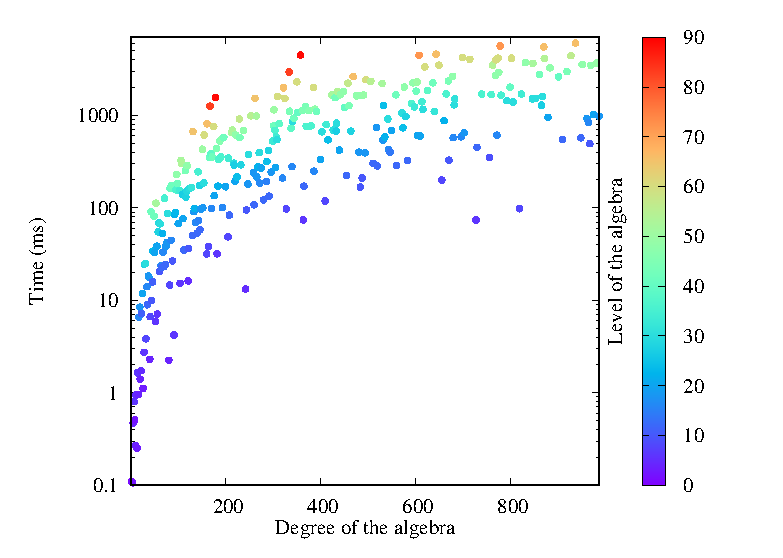
\includegraphics{benchmarks/lattice-h90/solve-h90-3.eps}
  \caption{Timings for computing decorated Kummer algebras $(A_m, \alpha_m)$ (logarithmic scale)
  with $p=3$.}
  \label{fig:solve-h90-3}
\end{figure}
\begin{figure}
  \centering
  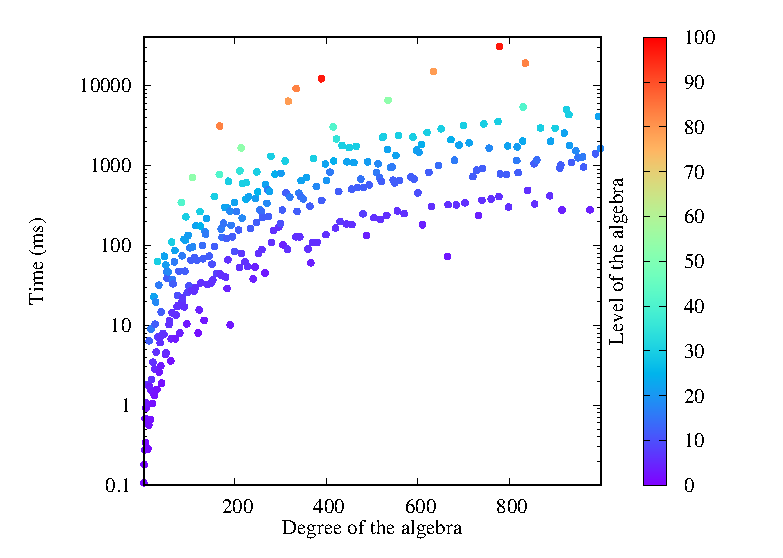
\includegraphics{benchmarks/lattice-h90/solve-h90-11.eps}
  \caption{Timings for computing decorated Kummer algebras $(A_m, \alpha_m)$ (logarithmic scale)
  with $p=11$.}
  \label{fig:solve-h90-11}
\end{figure}
In the complexity analysis of Proposition~\ref{prop:complexity-h90}, the level
of the algebra $A_m$ was bounded by its degree $m$, leading to a quasi-quadratic
complexity. However, we see in the timings that this bound is not relevant in
% TODO:
% =====
% Change that maybe? Not very smartly said. We could be more precise, and it is
% not even very true what we say...
practice. Indeed, the time results show that the level of the algebra has a
great impact on the timings: when the level is low, the computations are much
faster. In Figure~\ref{fig:level-12}, we selected only the computations that
occured on a fixed level $a=12$, and we see that in that case the time
complexity seems to be quasi-linear in the degree $m$.
\begin{figure}
  \centering
  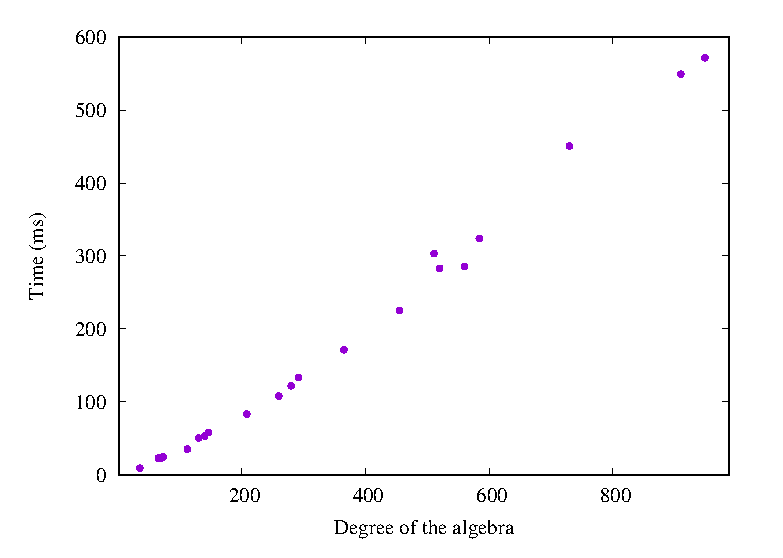
\includegraphics{benchmarks/lattice-h90/level-12.eps}
  \caption{Timings for computing decorated Kummer algebras $(A_m, \alpha_m)$ 
  with $p=3$ and with a given level $a=12$.}
  \label{fig:level-12}
\end{figure}
We also see that the characteristic $p$ has a small impact on the timings, as shown
in Figure~\ref{fig:degree-16} where we measure the timings for computing the
algebra $A_{16}$ and the corresponding solution of~\eqref{eq:h90-kummer}
$\alpha_{16}$, \ie we work with the fixed degree $m=16$ and we let the
characteristic be a prime number $p$ that grows from $3$ to $10^4$.
\begin{figure}
  \centering
  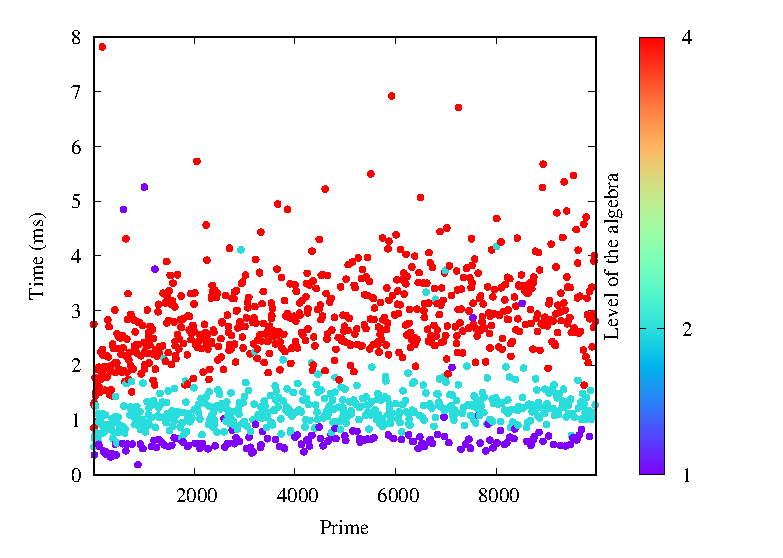
\includegraphics{benchmarks/lattice-h90/solve-h90-primes-degree-16.eps}
  \caption{Timings for computing decorated Kummer algebras $(A_{16},
  \alpha_{16})$ in characteristic $p$, with $p$ a prime number satisfying $3\leq
  p\leq 10^4$.}
  \label{fig:degree-16}
\end{figure}
The bottleneck of Algorithm~\ref{algo:decoration} appears to be the computation
of the $m$-th root extraction routine. When the decoration of two Kummer
algebras $A_m$ and $A_n$, with $m\mid n$, has been done; \ie when
Algorithm~\ref{algo:decoration} has been performed and solutions $\alpha_m$,
$\alpha_n$ are available, then the computation of the standard embedding
\[
  \mathbb{F}_{p^m}\emb\mathbb{F}_{p^n}
\]
is quite fast. In other words, Algorithm~\ref{algo:std-embed} is much faster
than Algorithm~\ref{algo:decoration}, which is a good thing because we only have
to call Algorithm~\ref{algo:decoration} once for each degree $m$, while
Algorithm~\ref{algo:std-embed} is called for each embedding computation, and
thus can be called several times with the same degree $m$. In
Figure~\ref{fig:embed-from-2}, we show the timings needed to compute embeddings
from $\mathbb{F}_{p^2}$ to $\mathbb{F}_{p^m}$, in the case where $p=3$, and for
every $4\leq m\leq 1000$ such that $p\nmid m$, $2\mid m$, and a suitable Conway
polynomial is available. Once again, the level of the destination algebra has an
important impact on the timings. 
\begin{figure}
  \centering
  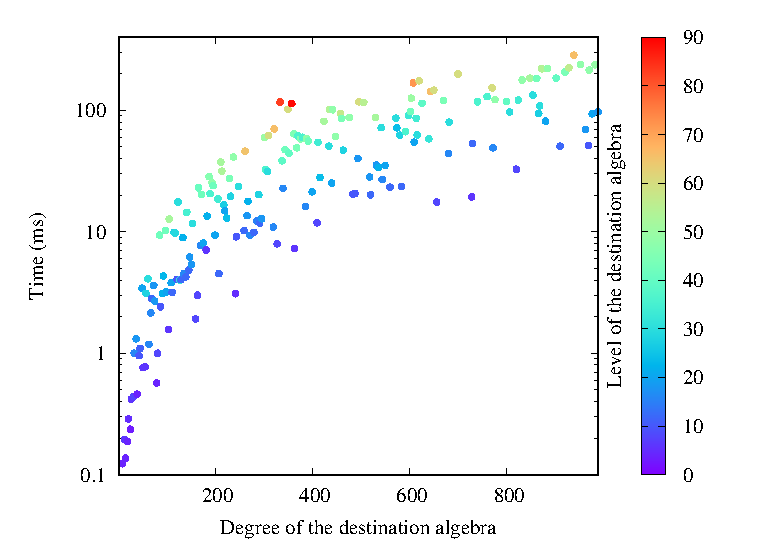
\includegraphics{benchmarks/lattice-h90/embed-from-degree-2.eps}
  \caption{Timings to compute the standard embedding from $\mathbb{F}_{p^2}$ to
  $\mathbb{F}_{p^m}$ (logarithmic scale), for $p=3$.}
  \label{fig:embed-from-2}
\end{figure}
We also measured the time needed to compute embeddings with extensions of a
fixed degree
\[
  \left[ \mathbb{F}_{p^{2m}}:\mathbb{F}_{p^m} \right] = 2
\]
in Figure~\ref{fig:embed-factor-2}, and we obtain similar results as in in
Figure~\ref{fig:embed-from-2} where the degree of the extension was varying but
the base field was fixed. Thus, it appears that the most important parameter
is the degree of the destination algebra.
\begin{figure}
  \centering
  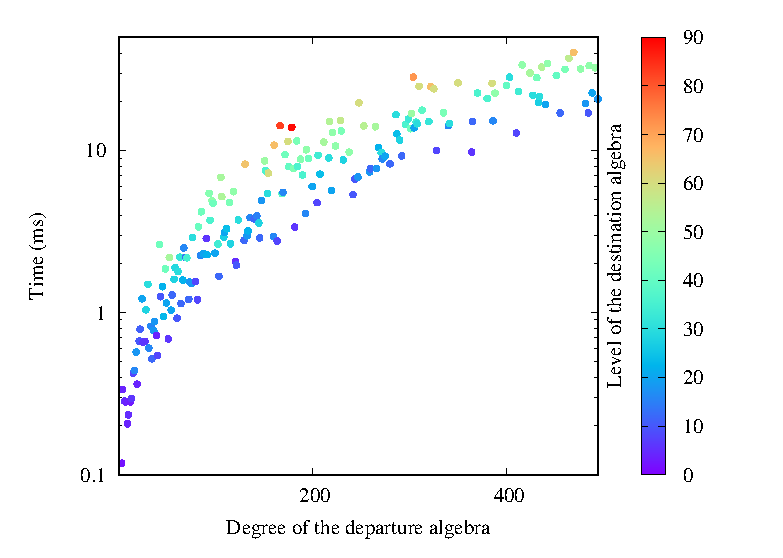
\includegraphics{benchmarks/lattice-h90/embed-factor-2.eps}
  \caption{Timings to compute the standard embedding from $\mathbb{F}_{p^m}$ to
  $\mathbb{F}_{p^{2m}}$ (logarithmic scale), for $p=3$.}
  \label{fig:embed-factor-2}
\end{figure}
Nevertheless, embedding computations seems to be faster with a small extension
degree. This is in particular shown in Figure~\ref{fig:embed-to-880}, where we
plot the timings for computing standard embeddings
\[
  \mathbb{F}_{p^d}\emb\mathbb{F}_{p^{880}}
\]
with $d\mid880$. The number $880$ was chosen because it is not divisible by
$p=3$ and because it has 20 different divisors, which is the maximum we can
obtain for numbers coprime to $3$ and less than $1000$. The number $560$ is
also suitable and produces similar results. We use logarithmic scale on the
abcissa axis because there is a greater number of small divisors.
\begin{figure}
  \centering
  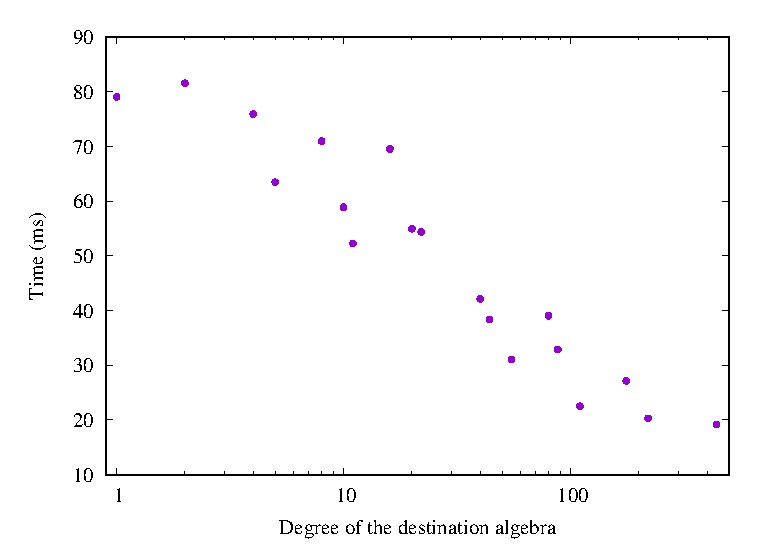
\includegraphics{benchmarks/lattice-h90/embed-to-degree-880.eps}
  \caption{Timings to compute the standard embedding from $\mathbb{F}_{p^d}$ to
  $\mathbb{F}_{p^{880}}$, for $p=3$ and $d\mid880$.}
  \label{fig:embed-to-880}
\end{figure}
The bottleneck of Algorithm~\ref{algo:std-embed} for computing a standard
embedding
\[
  \mathbb{F}_{p^m}\emb\mathbb{F}_{p^{n}}
\]
seems to be the powering $(\alpha_n)^{\frac{n}{m}}$ occuring in the destination algebra
$A_n$, which explains both the fact
that the algorithm is faster when the extension degree $\frac{n}{m}$ is smaller,
and the fact that the level of the destination algebra has an important impact
of the timings.
Again, we see in Figure~\ref{fig:embed-primes} that the impact of the
characteristic $p$ on the timings is minimal, compared to the other parameters.
\begin{figure}
  \centering
  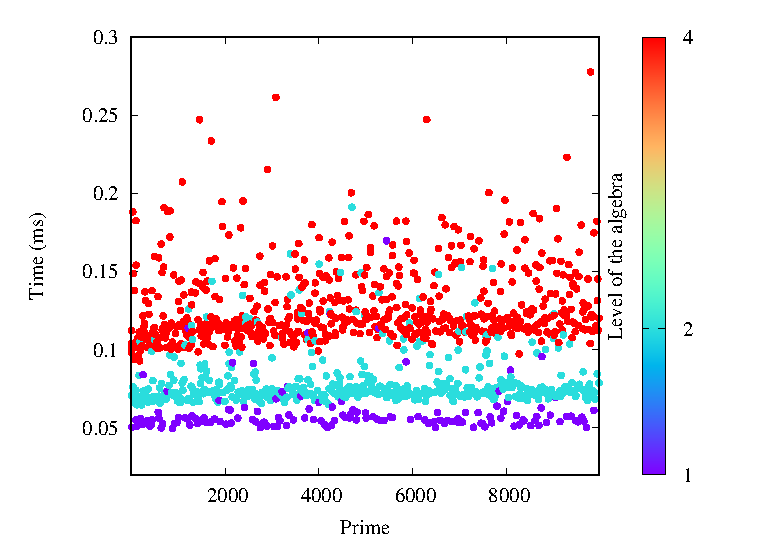
\includegraphics{benchmarks/lattice-h90/embed-primes-2-16.eps}
  \caption{Timings to compute the standard embedding from $\mathbb{F}_{p^2}$ to
  $\mathbb{F}_{p^{16}}$, for $p$ a prime number satisfying $3\leq p \leq 10^4$.}
  \label{fig:embed-primes}
\end{figure}

\section{Conclusion and perspectives}

In this chapter, we introduced a new idea to produce a lattice of compatibly
embedded finite fields, based on both Conway polynomials and Bosma-Canon-Steel
framework. Conway polynomials are used in many computer algebra systems, and
Bosma-Canon-Steel is used in Magma. Our idea exploits new techniques and is thus
interesting in itself. Furthermore, it also leads to a new family of (standard)
polynomials that can be used to define finite fields. Nevertheless, this new
family has no practical impact at the moment. Indeed, we can prove that
computing these polynomials is essentially equivalent to the computation of
Conway polynomials. Indeed, with our polynomials, one can recover a standard
solution $\alpha_m$ of~\eqref{eq:h90-kummer} and deduce the value
\[
  (\zeta_{p^a-1})^a.
\]
Then, by taking a $a$-th root, which is done in polynomial time in $m$, one can
find $\zeta_{p^a-1}$ and recover the associated Conway polynomial by computing a
minimal polynomial. This means that an efficient algorithm to compute our
standard polynomials would lead to an efficient algorithm to compute Conway
polynomials, which would be unexpected. We thus do not have great hope to find
such an algorithm, however the implemention presented in
Section~\ref{sec:implementation-std-lattices} is not the only possible way to
exploit our definitions. Indeed, it could be possible to loosen the assumption
that a cyclotomic lattice exists, and thus find a middle ground between the
rigidity of Conway polynomials and the flexibility of Bosma-Canon-Steel
framework, for example by lazily computing the roots of unity only when needed.
An orthogonal line of work would be to construct a complete lattice of
compatibly embedded finite fields, \ie working even with degrees that are not
coprime with the characteristic $p$ of the base field $\K$.
%
